%% SLMF.tex — ROUGH DRAFT
%% SLM Factory paper. Style follows draft.tex (acmart/sigconf) with the
%% structural conventions of arXiv:2604.09791 (Pioneer Agent): numbered
%% contributions, explicit formalism for the search space, per-section
%% "what it shows" readings of each table.
%%
%% Every number in this draft is traceable to a measurement in the repository.
%% Provenance is given in a LaTeX comment next to each table. Anything I could
%% not trace is marked \TODO and listed in the "Open questions" block at the
%% end of this file.

\documentclass[sigconf,10pt]{acmart}

\newcommand{\ceil}[1]{\lceil {#1} \rceil}
\newcommand{\floor}[1]{\lfloor {#1} \rfloor}

\usepackage{subcaption}
\usepackage{enumitem}
\usepackage{amsfonts,amsmath,amsthm}
\usepackage{graphicx}
\usepackage{booktabs}
\usepackage{multirow}
\usepackage{xcolor}
\usepackage{xurl}

\newcommand{\xref}[1]{\S\ref{#1}}
\newcommand{\tsk}[1]{\texttt{#1}}
\newcommand{\TODO}[1]{\textcolor{red}{\textbf{[TODO: #1]}}}

\AtBeginDocument{%
  \providecommand\BibTeX{{Bib\TeX}}}

\settopmatter{printacmref=false}
\renewcommand\footnotetextcopyrightpermission[1]{}

\newcommand{\squishlist}{\begin{itemize}[itemsep=1pt,parsep=2pt,topsep=3pt,partopsep=0pt,leftmargin=0em,itemindent=1em,labelwidth=1em,labelsep=0.5em]}
\newcommand{\squishend}{\end{itemize}}

\begin{document}

%% Title candidates. Current pick first; alternates kept for discussion.
\title{\huge{SLM Factory: Searching for the Smallest Model That Works on the Phone You Own}}
%\title{\huge{SLM Factory: Footprint-Constrained Closed-Loop Fine-Tuning of On-Device Language Models}}
%\title{\huge{From Prompt to Phone: Hardware-Constrained Autonomous Fine-Tuning of Small Language Models}}

\renewcommand{\shorttitle}{SLM Factory: Footprint-Constrained Closed-Loop Fine-Tuning}

%% \TODO{author block — names, affiliations, emails, ACM CCS concepts, keywords}
\author{Anonymous Author(s)}
\affiliation{%
  \institution{Anonymous Institution}
  \country{}
}

\begin{abstract}
Small language models are the only practical option for on-device deployment, but
choosing one is not a modelling problem so much as a budgeting problem: the model
must fit in the RAM and storage of a phone that already exists, and it must clear an
accuracy bar on one concrete task. Existing autonomous fine-tuning systems optimize
accuracy and treat compression as a downstream step; deployment footprint never enters
the search. We present \emph{SLM Factory}, a closed-loop agentic system that inverts the
objective: given a plain-English task description and a target device, it searches for
the \emph{smallest} deployable variant --- a (base model, quantization) pair drawn from a
pool of 27 measured variants --- that clears an accuracy goal calibrated against a local
teacher model. The system jointly searches training-pipeline space $\pi=(D,H,S)$ and
deployment-variant space, escalating up a size-ordered ladder only when a rung stagnates
and probing back down after convergence. Every quantized variant is scored on a real
GGUF build through \texttt{llama.cpp} rather than credited its full-precision score, and
a failed measurement is recorded as \emph{unmeasured} rather than as zero.
We evaluate on a ten-task suite organized by what fine-tuning is expected to buy, with
zero-shot baselines measured through each task's own scorer for two frontier APIs
(Claude Sonnet 5, DeepSeek v4 Flash) and for the local teacher. The fine-tuned on-device
student beats both frontier APIs on 9 of 10 tasks, with the largest margins on
format-bound tasks where the base model scores near zero: biomedical NER $0.000\to0.853$
against Claude's $0.165$, and nested semantic parsing $0.003\to0.599$ against $0.241$.
The two largest format-bound wins ship in under 1.3\,GB of weights.
We also report what the system did \emph{not} buy. Across the suite the median gain from
the entire iterative search after the first fine-tune is $+0.033$; the model ladder, not
the search, carries most runs; 81\% of the orchestrator's interventions were rolled back;
and two controlled A/B pairs show synthetic data is worth $+0.05$ per rung at one example
per class and indistinguishable from noise at thousands of real rows. We close with
measurement results that constrain how any of these numbers should be read: fine-tuning
under our stack is not bit-reproducible, and 4-bit quantization amplifies that
nondeterminism roughly fivefold.
\end{abstract}

\maketitle

%% ====================================================================
\section{Introduction}
\label{sec:intro}

A user who wants a language model to do one specific job on their phone faces a problem
that has nothing to do with modelling. They have a device with a fixed amount of usable
RAM and a storage budget they are willing to spend. Any model that does not fit is not a
worse option --- it is not an option. Within what fits, they want the best they can get on
their task, and, all else equal, they want the smallest thing that clears their bar, because
weights on a phone compete with photographs.

The research literature does not pose the problem this way. Work on parameter-efficient
fine-tuning~\cite{hu2021lora,dettmers2023qlora} and on post-training
quantization~\cite{frantar2022gptq,lin2024awq,dettmers2022llmint8} treats footprint
reduction as a transformation applied to a model that has already been chosen and trained.
Work on automated machine learning~\cite{feurer2015autosklearn,thornton2013autoweka,
feurer2019automl} searches hyperparameters against an accuracy objective on fixed hardware.
The recent line of agentic ML-engineering systems --- MLE-bench and its
successors~\cite{chan2024mlebench,nam2025mlgym}, execution-grounded search for GPU
kernels~\cite{chen2026kernelagent} and for scientific discovery~\cite{yamada2025aiscientist,
gottweis2025coscientist} --- and the closest prior system to ours, Pioneer
Agent~\cite{atreja2026pioneer}, all optimize a task metric and leave the deployment target
implicit. Pioneer Agent in particular formalizes autonomous fine-tuning as search over a
pipeline $\pi = (D,H,S)$ of dataset, hyperparameters, and strategy, and demonstrates
substantial gains --- but it trains through a hosted service, and nothing in its objective
knows how large the resulting artifact is.

We take the deployment budget as the primitive and the accuracy target as the constraint.
\emph{SLM Factory} accepts a free-text task description together with a target device
(``fine-tune a model for biomedical NER, deployed on my Galaxy S24 Ultra with 12\,GB RAM''),
resolves that device's usable RAM and storage from a local specification database with a
web-search fallback, filters a pool of 27 deployment variants --- nine base models from
135M to 4B parameters, each in \texttt{Q4\_K\_M}, \texttt{Q8\_0}, and \texttt{bf16} --- down
to those whose \emph{measured} weight bytes fit, and then runs a closed loop that searches
jointly over the training pipeline and the deployment variant. The loop curates a dataset,
trains one LoRA configuration, scores it on a frozen held-out set built before any training,
and asks a frontier orchestrator LLM for the next intervention; it rolls back on any
regression, escalates to the next larger variant when a rung stagnates, and, after clearing
its goal, probes \emph{downward} for a smaller variant that still clears it.

Two properties of the system are, we think, more consequential than the loop itself.

First, \textbf{evaluation is quantization-honest}. A run that will deploy a \texttt{Q4\_K\_M}
artifact scores a \texttt{Q4\_K\_M} artifact: the pipeline merges the adapter, converts to
GGUF, quantizes, and runs inference through \texttt{llama.cpp} on every iteration, with a
content-addressed cache and a reaping policy that keeps only the builds that set a new best.
No variant is ever credited a \texttt{bf16} score. Relatedly, a measurement that fails is
recorded as \emph{unmeasured} and rendered \texttt{n/a}; it is never recorded as $0.0$.
Conflating those two once credited fine-tuning with a fabricated $+0.85$ improvement in an
early NER run, which is the concrete incident behind the policy.

Second, \textbf{modelled quantities are structurally separated from measured ones}. Early
versions of the pool carried per-chip throughput multipliers and estimated peak inference
RAM, rendered in the same shape as measurements, and the hardware gates consumed them as
facts. The one estimate we later checked against reality was 20\% wrong. Those estimates are
now deleted rather than improved: the pool carries measured on-disk weight bytes and
published capability figures with their metric name, evaluation mode, and source URL
attached, and an unmeasured quantity gates nothing. This costs us the ability to make
throughput claims, and we make none.

We evaluate on a ten-task suite deliberately organized by \emph{what fine-tuning is expected
to buy} rather than by task family: in-distribution tasks where the base model can already
do the job and fine-tuning buys only format discipline; format-bound tasks where the model
knows the content but cannot produce the output contract; and tasks where the label is not
inferable from the input's surface form. For every task we measured zero-shot baselines
through the task's own prompt builder and scorer for Claude Sonnet 5, DeepSeek v4 Flash, and
our local teacher, so that a frontier-API cell and a student cell are computed by the same
code over the same frozen eval rows.

Our contributions:

\begin{enumerate}[leftmargin=*,itemsep=2pt]
\item \textbf{A footprint-constrained formulation of autonomous fine-tuning} (\xref{sec:formulation}).
We extend the pipeline-search formulation $\pi=(D,H,S)$ with a deployment-variant dimension
and invert the objective: minimize measured on-disk footprint subject to clearing a
calibrated accuracy goal, rather than maximize accuracy at fixed cost. The size-ordered
escalation ladder with post-convergence downward probing is the search procedure for that
objective.

\item \textbf{A quantization-honest, contamination-firewalled evaluation discipline}
(\xref{sec:system-eval}, \xref{sec:discussion}). Quantized variants are scored on real GGUF
builds; the held-out set is built before any training and owned by an agent that reports only
aggregates to the decision prompt; four independent firewall layers enforce train/eval
separation per row; failed measurements are \texttt{n/a}, never $0.0$.

\item \textbf{A goal that is calibrated rather than assumed} (\xref{sec:formulation-goal}).
The accuracy target is the local teacher's own score on the task's frozen eval set through
the task's own scorer, floored at $0.80$, with an audited ratchet that can raise it after
convergence. Goal provenance is printed in every run summary, so a floored goal and a
teacher-set goal are distinguishable at the same numeric value.

\item \textbf{A ten-task benchmark suite with frontier-API baselines measured through the
tasks' own scorers} (\xref{sec:suite}), organized by the expected mechanism of improvement,
with a refinement of that taxonomy: the predictive variable is not in- versus
out-of-distribution but whether the label is inferable from the input's surface form.

\item \textbf{Main results} (\xref{sec:results}). The fine-tuned on-device student beats both
frontier APIs zero-shot on 9 of 10 tasks; the single loss is function calling, where a 4B
base model already scores $0.848$. The largest wins are format-bound: \tsk{ner\_bc5cdr}
$0.000\to0.853$, \tsk{calendar\_json} $0.052\to0.875$, \tsk{topv2} $0.003\to0.599$.
Three of the ten winning artifacts are under 1.3\,GB, including two of those three
format-bound wins.

\item \textbf{Ablations and negative results that bound the value of the loop}
(\xref{sec:ablations}). Hyperparameter tuning alone matched the synthesis-enabled baseline
when the curriculum was already 2{,}700 real rows; two controlled A/B pairs show synthesis is
worth $+0.05$ to $+0.06$ per ladder rung at one real example per class and indistinguishable
from noise at thousands of rows; the median post-first-fine-tune search gain across the suite
is $+0.033$; and 81\% of the orchestrator's interventions were rolled back.

\item \textbf{Measurement-reliability results} (\xref{sec:reliability}). Training under
Unsloth is not bit-reproducible even with seeds, deterministic algorithms, and
\texttt{torch.compile} disabled. The resulting score noise is $\approx0.001$ in
\texttt{bf16}, $\approx0.006$ under \texttt{Q4\_K\_M}, and $\approx0.015$ on a 1{,}000-row
in-loop eval of a 151-class macro-F1 task. We derive a $\pm0.015$ noise floor from
triplicate probes and apply it throughout.
\end{enumerate}

%% ====================================================================
\section{Related Work}
\label{sec:related}

\paragraph{Autonomous fine-tuning and agentic ML engineering.}
Pioneer Agent~\cite{atreja2026pioneer} is the closest prior system and the direct
inspiration for our search formulation. It orchestrates a LangGraph state machine with a
frontier LLM, formalizes a training attempt as $\pi=(D,H,S)$, and searches that space with
Monte Carlo Graph Search, in a cold-start mode driven by a task description and a production
mode driven by judged inference failures. SLM Factory is an independent, open-backend
re-implementation of that architecture applied to a different objective. The differences that
matter are (i) the objective is footprint-constrained rather than accuracy-maximizing,
(ii) training runs on a standard open stack (Unsloth, PEFT, Transformers,
\texttt{llama.cpp}) on local and SLURM GPUs rather than through a hosted training service,
and (iii) deployment variant selection is inside the search rather than absent from it.
We also did not replicate production mode; \xref{sec:limitations} explains why.
More broadly, MLE-bench~\cite{chan2024mlebench} and MLGym~\cite{nam2025mlgym} establish that
LLM agents can execute substantial fractions of an ML workflow, and execution-grounded agent
search has produced strong results in GPU kernel optimization~\cite{chen2026kernelagent} and
automated research~\cite{yamada2025aiscientist,gottweis2025coscientist}.

\paragraph{AutoML and hyperparameter optimization.}
Classical AutoML~\cite{thornton2013autoweka,feurer2015autosklearn,feurer2019automl} and the
random- and grid-search baselines it displaced~\cite{bergstra2012random} optimize over a
predefined configuration space with a fixed dataset. Our search space is heterogeneous in
the same way Pioneer Agent's is --- data, optimization, and supervision interact
non-decomposably --- and additionally includes a discrete deployment dimension whose
elements differ in both capacity and numerical precision, which rules out a single fitted
scaling relation. Neural architecture search~\cite{elsken2019nas} shares the
hardware-awareness motivation; hardware-aware NAS~\cite{cai2019proxylessnas,
wu2019fbnet,tan2019mnasnet} is the closest methodological analogue to our ladder, but
searches architectures to train from scratch rather than selecting among pretrained
checkpoints and adapters.

\paragraph{Parameter-efficient fine-tuning and quantization.}
We fine-tune LoRA adapters~\cite{hu2021lora} on 4-bit-loaded base models in the manner of
QLoRA~\cite{dettmers2023qlora}, and deploy \texttt{Q4\_K\_M} and \texttt{Q8\_0} GGUF builds
through \texttt{llama.cpp}. The interaction we care about is not covered by the standard
PTQ literature~\cite{frantar2022gptq,lin2024awq,dettmers2022llmint8}: those papers measure
quantization degradation on a \emph{fixed} model, whereas our search chooses between a larger
model at lower precision and a smaller model at higher precision, which requires scoring both
as deployed. \xref{sec:reliability} reports a second-order effect that the PTQ literature
does not emphasize and that matters for any agentic loop scoring quantized artifacts:
4-bit rounding is a threshold operation, so it \emph{amplifies} upstream training
nondeterminism rather than merely adding its own.

\paragraph{Data-centric methods and synthetic data.}
Our data interventions descend from data-centric AI~\cite{northcutt2021confident,
mazumder2023dataperf} and from the ``quality over quantity'' line in instruction
tuning~\cite{zhou2023lima}. Synthetic supervision from a teacher model follows
self-instruct-style generation~\cite{wang2023selfinstruct} and knowledge
distillation~\cite{hinton2015distilling}, gated as in recent work showing that
\emph{filtering} matters more than raw teacher accuracy~\cite{bansal2025smallerweaker}.
We make that dependence explicit: a programmatic verifier runs before any teacher
judgement, and we report shadow-verification reject rates showing that generated-row
quality is a property of the task's output contract rather than of the generator
(\xref{sec:ablations-synthaudit}).

\paragraph{Contamination and evaluation integrity.}
Benchmark contamination in LLM evaluation is well
documented~\cite{sainz2023nlpcontamination,golchin2024timetravel}, and our tasks are drawn
from public benchmarks that frontier models have plausibly seen. We do not claim to have
solved this; we bound it structurally by pinning a held-out set before training, enforcing
per-row train/eval separation at four independent layers, and never letting the decision
prompt see a raw eval row. We make no claim about pretraining exposure, and we do not
measure it.

%% ====================================================================
\section{Problem Formulation}
\label{sec:formulation}

\subsection{Deployment variants}

A \emph{deployment variant} is a pair $v = (m, q)$ where $m$ is a pretrained base checkpoint
and $q \in \{\texttt{Q4\_K\_M}, \texttt{Q8\_0}, \texttt{bf16}\}$ is the on-device weight
format. The pool $\mathcal{V}$ contains nine base models spanning 135M to 4B parameters,
each expanded into all three formats, for $|\mathcal{V}| = 27$ independently selectable
variants (Table~\ref{tab:pool}). Each variant carries a footprint $s(v)$ in megabytes of
on-disk weights and a size bucket $\tau(v) \in \{0,1,2,3\}$ obtained by thresholding $s(v)$
at 750, 1500, and 2500\,MB.

Two things about this are deliberate. A variant is the unit of selection, not a base model:
the same checkpoint at two precisions can occupy different buckets, which is what allows the
search to trade precision against capacity. And $s(v)$ is a \emph{measured} quantity wherever
a real build exists. All 27 entries are measured; the bytes-per-parameter arithmetic that
would otherwise supply $s(v)$ was validated against those builds at $+4.8\%$ for
\texttt{Q4\_K\_M} and \texttt{bf16} and $-1.1\%$ for \texttt{Q8\_0}, with zero bucket changes,
so the fallback is trustworthy for a future pool addition.

\begin{table}[t]
\centering
\small
\caption{The variant pool: nine base models $\times$ three weight formats $=$ 27 deployment
variants. Sizes are measured on-disk weight bytes of real builds (SLURM job 37905779), not
estimates. Size buckets are computed per variant, so one checkpoint's formats can span
buckets.}
\label{tab:pool}
%% PROVENANCE: config/measured_metrics.json::_sizes; config/android_pool.py
\begin{tabular}{@{}lrrrr@{}}
\toprule
Base checkpoint & Params & \multicolumn{3}{c}{On-disk weights (MB)} \\
\cmidrule(l){3-5}
 & & \texttt{Q4\_K\_M} & \texttt{Q8\_0} & \texttt{bf16} \\
\midrule
SmolLM2-135M-Instruct        & 0.14B & 100.6  & 145.0  & 256.6  \\
gemma-3-270m-it              & 0.27B & 241.4  & 292.0  & 511.4  \\
SmolLM2-360M-Instruct        & 0.36B & 258.1  & 386.0  & 690.2  \\
Qwen3-0.6B                   & 0.6B  & 461.8  & 767.5  & 1433.7 \\
Qwen3.5-0.8B                 & 0.8B  & 516.8  & 795.0  & 1666.0 \\
Qwen3-1.7B                   & 1.7B  & 1223.0 & 2064.7 & 3875.3 \\
Qwen3.5-2B                   & 2B    & 1251.4 & 1980.5 & 4337.5 \\
Qwen3-4B-Instruct-2507       & 4B    & 2381.6 & 4082.1 & 7672.3 \\
Qwen3.5-4B                   & 4B    & 2654.5 & 4397.0 & 8908.0 \\
\bottomrule
\end{tabular}
\end{table}

\subsection{Device feasibility}

A device is summarized as $c = (R, G)$: usable RAM $R$ and storage budget $G$, both in
megabytes, resolved by fuzzy-matching the user's device string against a local phone
specification database, falling back to web search and an LLM extraction restricted to
emitting only device-specific values. The feasible set is
\begin{equation}
\mathcal{V}_c = \{\, v \in \mathcal{V} \;:\; s(v) \le G \;\wedge\; s(v) \le R \,\}.
\label{eq:feasible}
\end{equation}
Equation~\ref{eq:feasible} is a necessary condition, not a sufficient one: true peak
residency adds the KV cache and runtime overhead, so a variant that passes may still fail on
the device. We state it in this weak form on purpose. The alternative --- modelling peak
residency and throughput per chip --- is what we removed, because those estimates were
consumed by the gates as if they were measurements. When a real measurement exists for a
$(m,q,\text{chip})$ triple it gates \emph{additionally} on measured peak RSS and tokens per
second; an unmeasured triple reads as unknown and gates nothing. Throughput is never
estimated, and \texttt{min\_tok\_s} is never applied to an unmeasured candidate.

\subsection{Training pipelines}

Following~\cite{atreja2026pioneer}, a training pipeline is a triple $\pi = (D, H, S)$:
\squishlist
\item $D$ --- the dataset specification: the curriculum artifact version, its per-origin
composition (anchor / mined / synthetic), the rebuild plan that produced it, and the ordered
quality controls applied.
\item $H$ --- the hyperparameter configuration. Five fields are tunable: LoRA rank,
$\alpha$/rank ratio, weight decay, learning rate, and epoch count. Batch shape is derived by
the trainer from the device and is rejected if proposed; dropout is pinned at $0$.
\item $S$ --- the learning strategy: supervision format (direct target versus
chain-of-thought), the teacher used for annotation if any, loss masking
(\texttt{assistant\_only} throughout), and the scoring method.
\squishend
Let $\Pi$ denote the space of valid pipelines. For a variant $v$ and pipeline $\pi$,
$f(v,\pi) \in [0,1]$ is the score obtained by executing the full train-then-evaluate cycle
against the frozen held-out set under the task's declared metric, with the model
\emph{deployed as $v$} --- that is, quantized and served through \texttt{llama.cpp} when
$q \ne \texttt{bf16}$.

We evaluate a second quantity on every cycle. $g(v,\pi) \in [0,1]$ is the \emph{format
validity}: the fraction of predictions the task's scorer could parse at all. Reporting only
$f$ makes a model that reasons correctly and never emits a parseable answer
indistinguishable from one that reasons wrongly, which is a different failure with a
different fix. Nine of the ten tasks in our suite have a real parse step
(\xref{sec:suite}), and in the one case where the two diverged sharply --- a checkpoint
emitting stray reasoning tags --- $f$ collapsed while $g$ told the actual story.

\subsection{The objective}
\label{sec:formulation-objective}

Let $\theta$ be the accuracy goal (\xref{sec:formulation-goal}). The system solves
\begin{equation}
v^{*} = \arg\min_{v \,\in\, \mathcal{V}_c} \; s(v)
\quad \text{s.t.} \quad \max_{\pi \in \Pi} f(v, \pi) \;\ge\; \theta ,
\label{eq:objective}
\end{equation}
reporting the witnessing pipeline $\pi^{*} = \arg\max_{\pi} f(v^{*},\pi)$ alongside $v^{*}$.
This differs from the accuracy-maximizing objective of prior autonomous fine-tuning
work~\cite{atreja2026pioneer} in the direction of the optimization, and the difference is
what produces the ladder: the natural search procedure for
Equation~\ref{eq:objective} is to start at the smallest feasible variant, spend the pipeline
search there, and move up only when that rung cannot clear $\theta$.

Equation~\ref{eq:objective} is infeasible when no variant clears $\theta$. In that case the
system reports the lifetime-best $(v,\pi)$ across all rungs together with an explicit
non-convergence outcome and the reason (escalation ceiling, step budget, or wall clock).
We treat that as a result, not a failure to report: only three of the ten suite runs
converged, and the other seven --- two of which had convergence deliberately disabled so we
could measure their ceilings (\xref{sec:ablations-nostop}) --- report a lifetime best that is
still the number in Table~\ref{tab:main}. A system that reported only its converged runs
would report three tasks.

\subsection{Calibrating the goal}
\label{sec:formulation-goal}

A fixed accuracy target is either unreachable or trivial depending on the task, so $\theta$
is measured rather than chosen. Let $f_{\mathrm{T}}$ be the local teacher's score on the
task's own frozen eval set, computed through the task's own prompt builder and scorer. Then
\begin{equation}
\theta_0 = \max\bigl(0.80,\; f_{\mathrm{T}}\bigr),
\label{eq:theta}
\end{equation}
with $0.80$ an immutable floor. The orchestrator may \emph{lower} $\theta$ toward
$\theta_0$'s floor when remaining failures look like a capacity limit rather than a fixable
training deficiency, and is asked once per iteration whether to \emph{raise} it after a goal
is cleared. Raises must exceed the run's high-water mark by at least $0.005$ and are clamped
at $0.99$, so at most $(0.99-\theta_0)/0.005$ of them can occur and each requires clearing
the previous goal. A cleared goal is banked unconditionally before a raise is proposed, so
reaching for a stretch goal and missing it can never turn a successful run into a reported
failure.

One detail turns out to matter for reading results. A floored goal and a teacher-set goal
print the same number. In one early NER run, ``threshold 0.8000'' concealed a teacher that
had scored $0.0999$ --- the floor was doing all the work and the goal reflected what we
refused to go below rather than anything about the task. Goal provenance is therefore
recorded and printed: every run summary states whether the floor or the teacher set the
target, and what the teacher scored.

%% ====================================================================
\section{The SLM Factory System}
\label{sec:system}

\begin{figure}[t]
\centering
%% \TODO{FIGURE 1 — system architecture. Needs to be drawn. Suggested content:
%%   left: pre-graph device resolution + pool filtering (27 variants -> feasible set)
%%   center: the LangGraph loop (curate -> train -> evaluate -> [rollback] -> iterate)
%%     with iterate's four exits (train / curate / escalate / downward_probe)
%%   right: the size-ordered ladder with escalate arrows up and the downward probe
%%   bottom: the test-data agent as a firewall between the eval set and the decision prompt
%%   annotate: orchestrator = Claude Sonnet 5; teacher/judge = local Qwen3.6-35B-A3B vLLM }
\fbox{\parbox[c][3.2cm][c]{0.95\columnwidth}{\centering \TODO{Figure 1: system architecture}}}
\caption{SLM Factory architecture. A pre-graph stage resolves the target device and filters
the 27-variant pool on measured weight bytes. A LangGraph state machine then runs the shared
loop; \texttt{iterate} is the only node that chooses, and it chooses among two interventions
and two ladder moves. The test-data agent owns the frozen eval set and reports only
aggregates, so no raw held-out row reaches the decision prompt.}
\label{fig:arch}
\end{figure}

\subsection{Architecture}

The system (Figure~\ref{fig:arch}) is a LangGraph state machine over a single typed state
object, checkpointed to SQLite. Nodes are \texttt{task\_analysis}, \texttt{eval\_setup}, \texttt{model\_selection},
and then the shared loop \texttt{curate} $\to$ \texttt{train} $\to$ \texttt{evaluate} $\to$
(\texttt{rollback}) $\to$ \texttt{iterate}, from which four edges leave: back to
\texttt{train} (hyperparameter intervention), back to \texttt{curate} (data intervention),
\texttt{escalate} (move up a rung), or \texttt{downward\_probe} (search down after
convergence). Every edge is conditional and passes through a guard that can divert to
termination; there are no unconditional transitions.

The orchestrator is Claude Sonnet 5, used through a long-context beta for multi-day
trajectories. It is called at exactly four kinds of decision point: task planning, model
choice within a rung, the per-iteration intervention decision, and the stretch-goal question.
Everything else --- stagnation detection, rollback, budget enforcement, escalation --- is
deterministic, which is a deliberate allocation: plateauing is precisely when a run makes the
most \texttt{iterate} calls, so the rule that fires on a plateau is the one that must not
cost an API call or be overridable.

Two properties of the guard layer are worth stating because they changed run behaviour
materially. Wall-clock exhaustion \emph{skips} a node rather than interrupting it, so a long
training or evaluation step cannot start near a deadline and be killed mid-write. And any
exception whose class is defined in the provider SDK or its HTTP layer aborts the run rather
than degrading to a heuristic fallback, so an authentication or quota failure cannot produce
a run that silently limps along on score bands and reports a number.

The teacher, LLM judge, and synthesis generator are a single self-hosted
Qwen3.6-35B-A3B vLLM endpoint. We use one local model for all three roles for cost,
reproducibility, and contamination reasons, and the orchestrator is never a teacher: the
model that decides what to try must not also be the model that writes the training data, or
a run's outcome becomes uninterpretable.

\subsection{Task specifications}

Behaviour is per task, not per task family. Each benchmark is a module declaring a
\texttt{TaskSpec} with every field required and no defaults: its loader, mining sources,
metric, scorer, prompt builder, prediction extractor, failure-category function, eval
sampling policy, ordered quality controls, synthetic-row verifier, chain-of-thought flag,
and per-task caps on initial gold rows and eval rows. A decision nobody made for a task is
an import-time error rather than a silent runtime fallthrough.

This replaced dispatch on an abstract task type, and the replacement was not cosmetic. Under
the old design two classification tasks reported the same metric \emph{name} while computing
different quantities, and two structured-output tasks received an identical one-line
description in every teacher prompt --- omitting every convention that makes a calendar row
correct, so the verifier judging generated rows was judging its own guess. A descriptive
\texttt{family} tag survives for reports and model-selection hints and is enforced by test to
never be read as a dispatch key.

\subsection{Evaluation setup and contamination control}
\label{sec:system-eval}

\texttt{eval\_setup} builds the held-out set $\mathcal{E}$ \emph{before any training} and
freezes it for the run. $\mathcal{E}$ is a single flat sample, capped per task at 1{,}000
rows, drawn by the task's own sampling policy (label-balanced round-robin for closed-label
tasks, otherwise a plain draw). We cap at 1{,}000 because $\mathcal{E}$ is scored on every
iteration: at $n=1000$ the standard error on a proportion is about 1.5 points, below the
differences the search resolves, while an unbounded split would make each loop turn
proportionally slower for variance improvement that flattens out long before that. A short
eval set is accepted and logged as short.

Contamination is controlled at four independent layers. (1) After every acquisition path, any
training row whose normalized text matches a held-out row raises rather than being dropped ---
at load time an overlap is a loader bug. (2) Newly mined or generated rows are firewalled
per row, with each blocked row logged by provenance, label, length, and a hash of its
normalized text, never the text itself. (3) The firewall runs again after quality control,
because quality control can rewrite rows. (4) The label vocabulary is pinned from
$\mathcal{E}$ immediately after it is built, and every later stage may only \emph{drop} rows
outside it; no LLM may introduce a label. Separately, the trainer carves its own 12\%
validation split from the curriculum for best-checkpoint selection, so $\mathcal{E}$ is never
seen during training --- a three-way split, not two.

The decision prompt never sees a held-out row. A \emph{test-data agent} owns $\mathcal{E}$
and returns only aggregates: overall score, accuracy by difficulty bucket, the top failure
categories with counts, a diagnosis, and a suggested intervention. Difficulty labels are
assigned at \texttt{eval\_setup} by running the smallest and largest unique base checkpoints
zero-shot once: \emph{easy} if both are correct, \emph{medium} if only the larger is,
\emph{hard} if neither is. This is deliberately a measurement of the small-to-large capability
gap, which is the quantity the ladder exists to exploit.

Failure categories come from the task's own scorer, so a reported category names something
that was measured --- \texttt{wrong\_span\_boundaries} and \texttt{entities\_hallucinated}
for NER, \texttt{undeclared\_function} and \texttt{wrong\_call\_count} for function calling,
the real (gold, predicted) class confusion for closed-label tasks. A task that cannot define
an actionable taxonomy declares none and reports one honest aggregate. The previous design
collapsed every non-classification failure into a single literal category whose count equalled
the failure count the orchestrator already had; across a dozen iterations of one run the
orchestrator wrote paragraphs of reasoning about the behaviour of a constant and used it as
evidence.

\subsection{The ladder: selection, escalation, downward probing}
\label{sec:system-ladder}

Model selection supports five strategies, of which \texttt{smallest\_first} is the default
and the one used for every run reported here: begin at the smallest feasible variant, with no
throwaway probe, so the first train-and-evaluate cycle already uses the production
configuration. \texttt{largest\_first} establishes feasibility with one extra run;
\texttt{interpolation} fits score against log footprint over three probes;
\texttt{orchestrator\_choice} spends one API call with a prompt that explicitly optimizes for
resource efficiency rather than benchmark rank; \texttt{single\_model} disables the ladder
entirely and exists as the ablation control that isolates what the ladder buys.

\texttt{escalate} fires deterministically, on either of two conditions: no cumulative gain
above $0.02$ across the last 15 evaluations, or 30 evaluations on one variant without
clearing $\theta$. Stagnation is measured over an append-only evaluation history that
includes rolled-back attempts. Measuring it over the kept-score list instead --- which
rollback pops --- meant a mostly-regressing run never filled the window and the check
silently never fired. On escalation the system steps to the nearest higher non-empty size
bucket, asks the orchestrator to choose within it, archives the departing rung's full search
graph into the escalation history, frees the previous model's VRAM, and resets per-variant
search state while carrying forward the curriculum and the lifetime best score.

\texttt{downward\_probe} is the second half of Equation~\ref{eq:objective} and runs after
convergence: it searches for the smallest variant that still clears $\theta$, self-looping so
that each probe is one durable step and a crashed training process resumes without repeating
a paid decision. It unions the rungs it has tried with the rungs the main ladder already
trained, so it cannot re-select a variant whose true best is already known and retrain it with
a single fixed configuration that has no reason to beat the real search.

\subsection{Interventions}
\label{sec:system-interventions}

\texttt{iterate} is evaluated in a strict order, and the orchestrator is consulted only when
no deterministic rule applies: budget and wall-clock checks, then threshold handling (bank,
stretch-goal question, hardware re-gate, downward probe, or terminate), then forced escalation
on stagnation, then one tool-free LLM call. The call returns exactly one intervention.

\textbf{\texttt{hyperparameter}} holds the dataset fixed and changes one or more of the five
tunable fields, so the comparison is clean. An exact repeat of a tried
$(\text{dataset}, H)$ identity is rejected and replaced with a deterministic untried
neighbour; pruned and rolled-back trials count as tried. A non-hyperparameter intervention
carries forward the best prior configuration rather than reverting to a default --- previously
every data rebuild collapsed to the initial rank-16 default, so a rebuilt dataset was judged
with weaker hyperparameters than the incumbent, always regressed, and was always rolled back.
The data change could never be evaluated fairly.

\textbf{\texttt{data\_rebuild}} routes through \texttt{curate}, which has exactly two
sub-strategies, and a plan naming one that cannot add rows is rewritten rather than run:
\squishlist
\item \texttt{mine\_new\_real} adds real rows by a ladder --- re-read the task's own
unexhausted sources for a larger head slice (free: no provider call, no LLM column mapping,
no schema risk), then web discovery only once every known source is exhausted, then retire
for the run after two consecutive discovery rounds that contribute nothing. A source is
marked exhausted only when its loader returns \emph{fewer} rows than asked for, which is the
only reliable evidence a head slice has reached the end of a split.
\item \texttt{surgical\_synthesis} adds teacher-generated rows aimed at the failure categories
costing the most points, budgeted proportionally to each category's failure count and bounded
to $[25, 600]$ rows. A category already targeted whose count did not fall is marked
exhausted and skipped, so the run stops paying for something that is not responding.
\squishend
The curriculum is \emph{cumulative}: cold start loads the gold rows the loader returned,
every rebuild adds to what is on disk, and rows leave only via quality control or the
firewall. Nothing re-draws from a pool it has already drawn from, and there is no target
size. Three earlier mechanisms are absent for the same underlying reason --- resampling from
the pool the curriculum was built from (one traced rebuild resampled 3{,}308 rows of which 122
were novel), a universal gold refill to a target size (which re-selected the identical
$\sim$3{,}235 rows and honestly reported ``0 novel'' on eight consecutive rebuilds of one
run), and synthesis-fill padding to that same target. A rebuild that adds zero rows is now
logged as an error, because an intervention was chosen and the mechanism it named could not
do the thing it exists to do, so training this iteration would repeat the last one exactly.

\subsection{Synthesis: gated, contracted, twice-verified}
\label{sec:system-synthesis}

Synthetic data is refused for an entire run unless the teacher earns it. Before any
generation, the teacher is scored \emph{five-shot on this task's own frozen eval set through
this task's own scorer}, and if it scores below $0.80$ synthesis is disabled for the run. An
\emph{unmeasured} teacher is also refused: ``we could not check'' is not evidence of fitness,
and defaulting to allowed would mean a run that skipped the gate silently regained synthesis.
Five-shot rather than zero-shot, because five-shot is how synthesis actually prompts the
teacher --- on a format-bound task a zero-shot number mostly reports whether the teacher
guessed our output contract, and the gap is large: $0.113$ span-F1 zero-shot on BC5CDR
against $0.719$ with five demonstrations. Demonstrations are drawn from the training split
only, so measuring cannot leak a held-out row into a prompt that later scores it.

Generated rows pass two gates, exact first:
\[
\text{generate (5-shot)} \to \text{programmatic verify} \to \text{teacher verify} \to \text{QC}.
\]
The programmatic gate is free, cannot be fooled, and a row it rejects should never cost a
teacher call. Three tasks have one: function-call rows must parse, target a \emph{declared}
tool, and carry arguments present in its schema; calendar rows must additionally have parseable
datetimes, an end after its start, a 60-minute default for an unstated duration, and an event
resolving near the request's own reference instant; NER rows must have every span appear
verbatim in the row's own text with no duplicates. For the closed-label tasks there is no
answer to verify --- a generated row inherits a real anchor's label, so only the phrasing can
be wrong --- and for summarization correctness is not decidable by computation; both get the
teacher pass alone, and the code says so rather than implying a gate that does not exist.

Every synthesis and verification prompt is five-shot and is built from a \emph{task brief}
that the orchestrator authors once at cold start after being shown real rows: what the
benchmark is, its exact output contract, and its likely failure modes. Worked examples shown
to the teacher are always real rows from the task's own training split, never
orchestrator-invented, on the principle that a wrong example is worse than none.

\subsection{Rollback-first iteration and run health}

Any regression against the incumbent triggers \texttt{rollback}: pop the regressing score,
mark the newest search-graph node pruned, and restore from the best non-pruned node.
\texttt{rollback} never routes to \texttt{train} --- it routes to \texttt{iterate}, which is
forced to choose a \emph{different} action, because training is near-deterministic and
retraining the identical configuration would reproduce the same regression forever. Training
always restarts from the base model, never from a prior adapter, so a checkpoint's behaviour
is fully determined by the current iteration's dataset and configuration and rollback cleanly
restores prior behaviour without untangling accumulated updates.

A separate watchdog monitors \emph{across} iterations for patterns that mean a run cannot make
progress: two consecutive rebuilds adding zero rows; a curriculum that shrank by
$\ge$1{,}000 rows or $\ge$25\% in one iteration; two rebuild plans refused by the schema
validator; two consecutive total verification wipeouts; three mining attempts that saw
candidates and accepted none; two data-load failures. Every threshold requires a repeat or a
magnitude ordinary variance cannot explain, because a guard that fires on noise gets switched
off and a switched-off guard is worse than none. The watchdog exists because one run spent
7h42m and \$1.34 while all eight of its rebuilds added zero rows: each individual symptom
looked survivable and no component was watching for the repeat.

\subsection{Quantization-honest evaluation}

When the selected variant has $q \ne \texttt{bf16}$, \texttt{evaluate} merges the adapter,
converts to GGUF, quantizes, and scores through \texttt{llama.cpp}. Builds are cached under a
key derived from \emph{both} the weights reference and the quantization method: keying on the
weights reference alone made a \texttt{Q8\_0} rung silently reuse an earlier
\texttt{Q4\_K\_M} file, so two rungs scored identically. A cached file is reusable only when
its size and SHA-256 match a sidecar written after a real load. Builds are reaped unless
their iteration set a new best for the rung --- measured reuse was 0/138 on one run and 2/66
on another, at roughly 2.6\,GB apiece --- and a rollback needing a reaped build simply
rebuilds it.

The zero-shot baseline competes as a candidate at iteration 1. If no fine-tune beats the base
model, the base model is kept. This prevents shipping a fine-tune that is worse than doing
nothing, and it is not hypothetical: one task in our suite reached $+0.0000$ over 15
iterations, where the honest output of the loop is ``ship the base model''
(\xref{sec:results}).

\subsection{Durability}

Runs last days. A SQLite LangGraph checkpointer is the authority for graph position and a
JSON file is a human-readable mirror; if the mirror records progress that SQLite does not
have, the run aborts rather than silently restarting. A graph-topology descriptor is compared
on resume, so a checkpoint written by a different graph shape is rejected. Datasets, eval
sets, checkpoints, and training outputs are written atomically. Under SLURM the batch shell
forwards a pre-timeout signal, waits for both checkpoints to land, verifies durable resume
state, and only then requeues into the same run directory, producing segment rollover with
continuous progress instead of a terminal run; the wall-clock guard is aggregate across
segments, so a resumed run inherits its predecessor's elapsed time. A file-locked,
append-only cost ledger is shared by the runner, forked acquisition processes, and spawned
CUDA workers. The end-of-run report is registered with \texttt{atexit}, so a cancelled or
crashed run still prints its per-iteration table, curriculum growth ledger, attribution
breakdown, and teacher-fitness verdict.

%% ====================================================================
\section{Benchmark Suite}
\label{sec:suite}

We organize tasks by the mechanism through which fine-tuning is expected to help, because
that is what predicts the shape of the result. Table~\ref{tab:suite} gives the suite.

\begin{table}[t]
\centering
\small
\caption{The ten-task suite, grouped by the expected mechanism of improvement. Metrics are the
string the task's own scorer returns.}
\label{tab:suite}
%% PROVENANCE: tasks/*.py TaskSpec; docs/PIPELINE.md §6.5
\begin{tabular}{@{}lll@{}}
\toprule
Task & What it is & Metric \\
\midrule
\multicolumn{3}{@{}l}{\emph{In-distribution} --- FT buys format discipline} \\
\tsk{gsm8k}      & grade-school math      & \tsk{exact\_match} \\
\tsk{dialogsum}  & dialogue summarization & \tsk{rouge\_l} \\
\addlinespace
\multicolumn{3}{@{}l}{\emph{Format-bound} --- knows the content, not the contract} \\
\tsk{xlam\_bfcl}     & function calling         & \tsk{ast\_arg\_match} \\
\tsk{calendar\_json} & text $\to$ calendar JSON & \tsk{ast\_arg\_match} \\
\tsk{ner\_bc5cdr}    & biomedical NER           & \tsk{span\_f1} \\
\tsk{multiconer}     & 33-class fine-grained NER & \tsk{micro\_f1} \\
\tsk{topv2}          & nested intent/slot parse & \tsk{exact\_match} \\
\addlinespace
\multicolumn{3}{@{}l}{\emph{Label not inferable from surface form}} \\
\tsk{clinc150}   & 150-class intent        & \tsk{macro\_f1} \\
\tsk{sms\_spam}  & spam, minority class    & \tsk{minority\_f1} \\
\tsk{goemotions} & 28-label emotion        & \tsk{ekman\_macro\_f1} \\
\tsk{gec\_bea19} & grammatical error corr. & \tsk{errant\_f05} \\
\bottomrule
\end{tabular}
\end{table}

\paragraph{In-distribution.} The base model can already do the task; fine-tuning buys format
discipline. Prediction: good baseline, small delta.

\paragraph{Format-bound.} The model knows the content but cannot produce the output contract.
Prediction: near-zero baseline, large delta. This is the group the on-device case is about,
because a phone-sized model that can be taught a contract is worth more than a frontier model
that must be called over the network to produce one.

\paragraph{Label not inferable from surface form.} We originally called this group
``out-of-distribution'' and predicted a poor baseline. The data corrected us, and the
correction is worth stating because it is the most useful thing the taxonomy taught us.
\tsk{clinc150}'s label \emph{is} the utterance's meaning, so any competent model reads it off
directly: the teacher scores $0.877$ and the first fine-tune adds little. \tsk{routerbench}'s
label is \emph{another model's} correctness, which is unreadable from the input, so its
baseline looked mid-range but was noise and its ceiling is capped by label noise. The
predictive variable is therefore not distributional novelty but whether the label is a
function of the input's surface form. Under that relabelling \tsk{clinc150} is an
in-distribution control that shows the loop correctly doing little when there is little to do.

\paragraph{Protocol.} Every number reported for this suite is computed through the task's own
prompt builder, prediction extractor, and scorer over the same frozen eval set the runs used,
so a frontier-API cell, a teacher cell, and a student cell are directly comparable. Zero-shot
API baselines were measured with reasoning disabled on both providers over full eval sets via
batch APIs, at a total cost of \$9.67 for 20 cells with zero errors and format validity
between $0.95$ and $1.00$. Paper numbers for students come from a standalone report script
over a large report split rather than from the in-loop 1{,}000-row figure, for reasons given
in \xref{sec:reliability}. We treat any single-run difference below $\pm0.015$ as unmeasured
(\xref{sec:reliability}).

\paragraph{Caveats on individual cells.} Three are load-bearing.
\tsk{multiconer}'s $0.639$ clears the $0.610$ published state of the art but was trained on 27
of 33 entity types --- the 5{,}000-row cap was a prefix slice of an unshuffled file, so six
classes had zero training mentions while hundreds of examples of each sat unused. Micro-F1 is
sound; the macro-F1 report metric has six classes pinned at zero by construction.
\tsk{dialogsum} uses max-over-three-references ROUGE, so $0.482$ is not comparable to the
single-reference published figure of $0.395$. And all five of the 09-2026 suite runs bypassed
the teacher fitness gate: the teacher failed the $0.80$ gate on every one and synthetic data
was allowed anyway, so those are not clean results in the gate's own terms.
Those five results should be read as measuring the loop with synthesis permitted
unconditionally, which is a weaker protocol than the one the system normally enforces.

%% ====================================================================
\section{Experiments}
\label{sec:results}

\subsection{Setup}

All runs execute on a SLURM cluster with L40S or RTX 6000 Ada nodes, one GPU per run.
Orchestration is Claude Sonnet 5. The teacher, judge, and generator is a self-hosted
Qwen3.6-35B-A3B vLLM endpoint for nine of the ten suite runs; \tsk{xlam\_bfcl} is the
exception and used \texttt{deepseek-v4-flash} as its teacher, which we flag here because it
makes that one run's synthesis non-comparable to the other nine and because it is what
produced the cost outlier in Table~\ref{tab:cost}. Training is LoRA over a 4-bit-loaded base
through Unsloth and PEFT, always from the base checkpoint, with completion-only loss and
best-validation checkpointing. The default starting configuration is rank 16, $\alpha$ 32, dropout 0, weight
decay 0.01, learning rate $2\times10^{-4}$, 3 epochs, micro-batch 8. Model selection is
\texttt{smallest\_first} throughout.

The escalation ladder actually traversed by the suite runs has five rungs, which we index R1
through R5: R1 SmolLM2-360M-Instruct@\texttt{Q4\_K\_M} (258\,MB), R2
Qwen3.5-0.8B@\texttt{Q4\_K\_M} (517\,MB), R3 Qwen3-1.7B@\texttt{Q4\_K\_M} (1{,}223\,MB), R4
Qwen3-4B-Instruct-2507@\texttt{Q4\_K\_M} (2{,}382\,MB), R5
Qwen3-4B-Instruct-2507@\texttt{Q8\_0} (4{,}082\,MB). Two tasks stopped at R3.
%% \TODO{AUTHORS: state the device string and RAM/storage budget used for these runs here.
%%   The top rung needs a >=4 GB weight budget, so the constraint should be explicit.}

\subsection{Main results}

\begin{table*}[t]
\centering
\small
\caption{Main results. All cells computed through the task's own scorer over the same frozen
eval set. \textbf{Bold} marks the winner across the API, teacher, and best-student columns.
\emph{Student 0-shot} and \emph{First fine-tune} are the winning variant's own scores, so
those three columns tell one model's story: how much of the improvement came from the first
training run and how much from the search after it. Footprint is the measured on-disk weight
bytes of that variant. \emph{Best student} is the lifetime best across all rungs, and the
winning variant is the one that scored it --- which is not always the rung the run finally
stopped on; see the discussion of \tsk{sms\_spam} below.}
\label{tab:main}
%% PROVENANCE: docs/Evan's Notes/09-16-baselines-ablations-and-probes.md Part I.1
%% API data: logs/probes/api-baselines.json. Run logs: logs/slurm/Final Runs/.
\footnotesize
\begin{tabular}{@{}llrrrrrrlr@{}}
\toprule
Task & Metric & \shortstack[r]{Claude\\Sonnet 5} & \shortstack[r]{DeepSeek\\v4 Flash} & \shortstack[r]{Teacher\\0-shot} & \shortstack[r]{Student\\0-shot} & \shortstack[r]{First\\fine-tune} & \shortstack[r]{Best\\student} & Winning variant & \shortstack[r]{Footprint\\(MB)} \\
\midrule
\tsk{clinc150}      & \tsk{macro\_f1}         & 0.9212 & 0.9067 & 0.8771 & 0.7663 & 0.9010 & \textbf{0.9372} & Qwen3-4B-Instruct@\texttt{Q8\_0} & 4082 \\
\tsk{sms\_spam}     & \tsk{minority\_f1}      & 0.9538 & 0.8561 & 0.8641 & 0.0000 & 0.7071 & \textbf{0.9609} & Qwen3-1.7B@\texttt{Q4\_K\_M}     & 1223 \\
\tsk{calendar\_json}& \tsk{ast\_arg\_match}   & 0.5140 & 0.5047 & 0.2037 & 0.0523 & 0.8168 & \textbf{0.8748} & Qwen3.5-2B@\texttt{Q4\_K\_M}     & 1251 \\
\tsk{xlam\_bfcl}    & \tsk{ast\_arg\_match}   & 0.8790 & \textbf{0.8960} & 0.8660 & 0.8480 & 0.8510 & 0.8740 & Qwen3-4B-Instruct@\texttt{Q8\_0} & 4082 \\
\tsk{ner\_bc5cdr}   & \tsk{span\_f1}          & 0.1647 & 0.1277 & 0.1321 & 0.0000 & 0.8357 & \textbf{0.8532} & Qwen3.5-2B@\texttt{Q4\_K\_M}     & 1251 \\
\tsk{goemotions}    & \tsk{ekman\_macro\_f1}  & 0.5062 & 0.4481 & 0.4227 & 0.3775 & 0.5979 & \textbf{0.5979} & Qwen3-4B-Instruct@\texttt{Q8\_0} & 4082 \\
\tsk{gec\_bea19}    & \tsk{errant\_f05}       & 0.4758 & 0.5176 & 0.5014 & 0.4352 & 0.5358 & \textbf{0.5647} & Qwen3-4B-Instruct@\texttt{Q8\_0} & 4082 \\
\tsk{multiconer}    & \tsk{micro\_f1}         & 0.4912 & 0.4283 & 0.4306 & 0.2844 & 0.5692 & \textbf{0.6388} & Qwen3-4B-Instruct@\texttt{Q8\_0} & 4082 \\
\tsk{dialogsum}     & \tsk{rouge\_l}          & 0.3342 & 0.3272 & 0.2843 & 0.2721 & 0.4817 & \textbf{0.4817} & Qwen3-4B-Instruct@\texttt{Q8\_0} & 4082 \\
\tsk{topv2}         & \tsk{exact\_match}      & 0.2410 & 0.1450 & 0.0230 & 0.0030 & 0.5340 & \textbf{0.5990} & Qwen3-4B-Instruct@\texttt{Q8\_0} & 4082 \\
\bottomrule
\end{tabular}
\end{table*}

\paragraph{The fine-tuned on-device student beats both frontier APIs on 9 of 10 tasks.}
The single loss is \tsk{xlam\_bfcl}, at $0.8740$ against Claude's $0.8790$ and DeepSeek's
$0.8960$, and it is the honest low point of the suite: a 4B model already calls functions at
$0.848$ out of the box, so there was little for the loop to win and it did not win it.

\paragraph{The loop wins hardest where the base model cannot do the task at all.}
\tsk{ner\_bc5cdr} goes $0.0000 \to 0.8532$ against Claude's $0.1647$; \tsk{calendar\_json}
$0.0523 \to 0.8748$ against $0.5140$; \tsk{topv2} $0.0030 \to 0.5990$ against $0.2410$.
These are exactly the format-bound extraction and structured-output tasks the on-device case
is about --- the frontier models know the content and cannot be made to emit the contract
without being told, and a fine-tuned 1.3\,GB model can be.

\paragraph{Three of the ten best results come from an artifact under 1.3\,GB, and two of them
are the largest format-bound wins} (Figure~\ref{fig:pareto}). \tsk{ner\_bc5cdr} and
\tsk{calendar\_json} both score their best on Qwen3.5-2B@\texttt{Q4\_K\_M} at 1{,}251\,MB,
and \tsk{sms\_spam} on Qwen3-1.7B@\texttt{Q4\_K\_M} at 1{,}223\,MB. The other seven need the
ladder's top rung at 4{,}082\,MB.

We want to be precise about what this does and does not show. The footprint-constrained
objective delivers a genuinely small artifact on the tasks where fine-tuning teaches an
output contract, and it does not on the tasks where the score is bounded by model capacity or
by label noise. The central claim of this paper is therefore about the format-bound group
specifically, and we state it that way rather than averaging over all ten.

\paragraph{One of these three is a best score the run did not ship.} \tsk{sms\_spam} peaked at
$0.9609$ on R3 and kept climbing the ladder to R5, where it scored $0.9490$ --- so the run's
final deployed variant was 3.3$\times$ larger and slightly worse than its own best. This is
exactly what the post-convergence downward probe exists to prevent, and it did not run,
because the probe is unreachable under the \texttt{smallest\_first} strategy every suite run
used. It is a gap between the objective we state in Equation~\ref{eq:objective} and the
behaviour we shipped, not a property of the objective, and we flag it as such in
\xref{sec:limitations} rather than quietly reporting the better number.

\begin{figure}[t]
\centering
%% \TODO{FIGURE 2 — accuracy vs measured footprint, per task, one marker per ladder rung,
%%   with the frontier-API scores drawn as horizontal reference lines. This is the figure
%%   that makes the footprint-constrained objective legible and we do not have it yet.
%%   Data: each run log's per-tier "Model Improvement Report" + measured_metrics.json sizes.}
\fbox{\parbox[c][4cm][c]{0.95\columnwidth}{\centering \TODO{Figure 2: score vs measured footprint, per rung, all ten tasks}}}
\caption{Best score achieved at each ladder rung against that rung's measured on-disk
footprint, with frontier-API zero-shot scores as horizontal references. The knee of each
curve is what Equation~\ref{eq:objective} is trying to find.}
\label{fig:pareto}
\end{figure}

\subsection{Where the search actually paid}

Table~\ref{tab:gain} reports, per task, the rung whose \emph{search} gained most --- which is
rarely the rung that scored highest.

\begin{table}[t]
\centering
\small
\caption{The highest-gain rung per task. ``Search gain'' is best-at-rung minus
first-fine-tune-at-rung: what iteration bought after the first training run, not what
fine-tuning bought over the base model.}
\label{tab:gain}
%% PROVENANCE: 09-16 note, Part I.1 "Where the search actually paid"
\begin{tabular}{@{}llrrr@{}}
\toprule
Task & Highest-gain rung & \shortstack[r]{First\\FT} & \shortstack[r]{Search\\gain} & \shortstack[r]{Also best\\scoring?} \\
\midrule
\tsk{clinc150}       & R4 Qwen3-4B@Q4   & 0.8112 & $+0.1082$ & no \\
\tsk{sms\_spam}      & R3 Qwen3-1.7B@Q4 & 0.7071 & $+0.2539$ & \textbf{yes} \\
\tsk{calendar\_json} & R1 SmolLM2-360M  & 0.4953 & $+0.1738$ & no \\
\tsk{xlam\_bfcl}     & R1 gemma-3-270m  & 0.0050 & $+0.0410$ & no\,$^{\dagger}$ \\
\tsk{ner\_bc5cdr}    & R1 SmolLM2-360M  & 0.6885 & $+0.0808$ & no \\
\tsk{goemotions}     & R1 SmolLM2-360M  & 0.4102 & $+0.1560$ & no \\
\tsk{gec\_bea19}     & R4 Qwen3-4B@Q4   & 0.5149 & $+0.0359$ & no \\
\tsk{multiconer}     & R3 Qwen3-1.7B@Q4 & 0.4546 & $+0.0749$ & no \\
\tsk{dialogsum}      & R4 Qwen3-4B@Q4   & 0.4462 & $+0.0339$ & no \\
\tsk{topv2}          & R1 gemma-3-270m  & 0.2080 & $+0.2170$ & no \\
\bottomrule
\multicolumn{5}{@{}p{0.95\columnwidth}@{}}{\footnotesize $^{\dagger}$ Discount this row
entirely: its highest-gain rung is a 270M model with format validity $0.373$, so $+0.041$ is
movement between two scores that were never usable.}
\end{tabular}
\end{table}

\paragraph{The search pays where the model starts furthest from the ceiling, which is almost
never where the run ends up.} Only \tsk{sms\_spam} peaks in gain and in score at the same
rung. On five of ten the gain peaks at R1, the smallest model in the ladder. Once a run
escalates, the larger model's \emph{first} fine-tune already lands near its plateau, which is
why the search-gain column is so small at the top rungs.

\paragraph{Almost all of the improvement is the first fine-tune, not the search after it.}
Differencing Table~\ref{tab:main}'s last two numeric columns gives what the search bought
after the first training run at the winning rung: the median is $+0.033$ and eight of ten
tasks sit at or below $+0.07$. Two tasks --- \tsk{goemotions} and \tsk{dialogsum} --- are at
exactly $+0.0000$, meaning the winning rung's first training run was already its best. The
one large exception, \tsk{sms\_spam} at $+0.2539$, is a collapse being repaired rather than a
model improving (\xref{sec:ablations-scarcity}). What the ladder contributes shows up as the
difference \emph{between} rungs, not in this column, and Table~\ref{tab:gain} shows the same
thing from the other side: where the search gains most is not where the run ends up.

\paragraph{81\% of the orchestrator's interventions were discarded.} On the \tsk{clinc150}
no-convergence rerun --- 91 iterations across all five rungs --- the end-of-run attribution
reads: hyperparameter $+0.1785$ from 9 of 37 attempts kept, \texttt{mine\_new\_real}
$+0.1353$ from 3 of 23, \texttt{surgical\_synthesis} $+0.0432$ from 4 of 25. That is 16 of 85
interventions kept, a 19\% hit rate. This is one run rather than an average over the suite,
and we report it because it is the operating characteristic of the loop rather than an
aberration: the rollback-first policy is what lets a 19\% hit rate produce monotone progress,
and a system with this hit rate and \emph{without} rollback would move backwards.

\subsection{Cost and wall clock}

\begin{table}[t]
\centering
\small
\caption{Per-run resource use for the suite. Orchestrator cost is Claude Sonnet 5 API spend;
local teacher, judge, and generator calls are free by construction, which is why the local-call
column is large and the dollar column is not. The \tsk{xlam\_bfcl} row is the one run that used
a paid API teacher instead, and it is why the other nine do not.}
\label{tab:cost}
%% PROVENANCE: per-run "cost:" summary lines in logs/slurm/Final Runs/*.out
\begin{tabular}{@{}lrrrr@{}}
\toprule
Task & \shortstack[r]{Orch.\\calls} & \shortstack[r]{Orch.\\cost} & \shortstack[r]{Local\\calls} & Outcome \\
\midrule
\tsk{calendar\_json} &  68 & \$1.89 &  1{,}798 & converged \\
\tsk{ner\_bc5cdr}    &  62 & \$3.43 & 17{,}831 & converged \\
\tsk{xlam\_bfcl}     &  75 & \$4.83$^{\ddagger}$ & --- & converged \\
\tsk{dialogsum}      &  83 & \$5.04 & 21{,}236 & ceiling \\
\tsk{gec\_bea19}     &  80 & \$5.19 & 22{,}270 & ceiling \\
\tsk{sms\_spam}      &  90 & \$5.23 &  9{,}842 & ceiling$^{\S}$ \\
\tsk{goemotions}     &  91 & \$6.04 & 20{,}794 & ceiling \\
\tsk{multiconer}     & 101 & \$6.60 & 27{,}704 & ceiling \\
\tsk{clinc150}       &  95 & \$6.92 & 14{,}467 & ceiling$^{\S}$ \\
\tsk{topv2}          & 112 & \$7.73 & 46{,}049 & ceiling \\
\bottomrule
\multicolumn{5}{@{}p{0.95\columnwidth}@{}}{\footnotesize $^{\ddagger}$ Orchestration only.
This run additionally spent \$38.05 on \texttt{deepseek-v4-flash} synthesis --- 18{,}145
generation calls emitting 52.7M output tokens --- because the thinking-disable flag was sent
only on the local path, so the API teacher reasoned on every generated row. That is
$7.9\times$ the run's own orchestration budget and more than the other nine runs' orchestration
combined. See \xref{sec:ablations-teacher}. $^{\S}$ Convergence deliberately disabled
(\xref{sec:ablations-nostop}).}
\end{tabular}
\end{table}

Table~\ref{tab:cost} gives per-run resource use.

\paragraph{An end-to-end run costs single-digit dollars of orchestration.} Orchestration is
62--112 API calls and \$1.89--\$7.73 per run, against tens of thousands of free local
teacher, judge, and inference calls. The dominant real cost is GPU wall clock, which runs
from roughly six hours to multiple days per task depending on how far up the ladder the run
climbs. \TODO{add a wall-clock column --- the numbers are in the SLURM accounting, not in the
log lines I extracted}

\paragraph{The one run that used a paid API teacher spent $7.9\times$ its own orchestration
budget on synthesis alone}, and produced the suite's only loss against the frontier APIs.
The two facts are not causally linked --- \tsk{xlam\_bfcl} is a hard case for the loop
regardless (\xref{sec:results}) --- but the cost was pure waste: the API teacher reasoned on
every generated row because our client sent the thinking-disable flag only on the local path.
This is the strongest single argument for the local-teacher design, and it was not a design
insight. It was a bug in our own client, and \xref{sec:ablations-teacher} reports what it
cost us in interpretability as well as in dollars.

%% ====================================================================
\section{Ablations}
\label{sec:ablations}

\subsection{Does synthetic data help at all?}
\label{sec:ablations-nosynth}

The cleanest comparison in the suite is a \tsk{ner\_bc5cdr} arm that refused synthesis for the
whole run and happened to select the same R1 model as the baseline:

\begin{center}
\small
\begin{tabular}{@{}lrrr@{}}
\toprule
Arm & Iterations & R1 best & Synthesis rounds \\
\midrule
baseline           & 26 & 0.7694 & 2 \\
no-synth           & 30 & \textbf{0.7756} & 0 \\
\bottomrule
\end{tabular}
\end{center}

Hyperparameter tuning alone beat the synthesis-enabled baseline, on one run with four more
iterations and the same mined rows. The difference is inside the noise floor and should be
read as ``no measured difference,'' which is itself the finding. \xref{sec:ablations-scarcity}
explains why: this curriculum was 2{,}700 rows of which 101 were synthetic, so synthesis
never had room to matter.

\subsection{Does synthetic data earn its keep when real data is scarce?}
\label{sec:ablations-scarcity}

Two A/B pairs test that hypothesis by starving a run of real data and changing nothing else.
Each pair's arms differ \emph{only} in whether synthesis is allowed; a registry test enforces
that by diffing both launchers against the task's baseline. Both pin the goal at $0.99$ so
neither arm can converge early, refuse mining so the cap cannot be read back out of the same
corpus, and lower the curriculum viability floor because a curriculum this small is exactly
what that guard exists to catch.

\begin{table}[t]
\centering
\small
\caption{Scarcity ablation. Per-rung best score for the no-synthesis arm (A) and the
synthesis-enabled arm (B). \tsk{sms\_spam} is capped at 100 real rows ($\approx$50 per class,
binary); \tsk{clinc150} at 151 rows drawn round-robin, which lands exactly one example on
every intent.}
\label{tab:scarcity}
%% PROVENANCE: 09-16 note, Part III.1 and III.2. Jobs 40128751/40126479 and 40175896/40175895.
\begin{tabular}{@{}llrrrr@{}}
\toprule
Task & Rung & 0-shot & Arm A & Arm B & $\Delta$ \\
\midrule
\multirow{5}{*}{\tsk{sms\_spam}}
& R1 SmolLM2-360M   & 0.2354 & 0.6369 & \textbf{0.9350} & $\mathbf{+0.2981}$ \\
& R2 Qwen3.5-0.8B   & 0.2272 & 0.9349 & 0.9569 & $+0.0220$ \\
& R3 Qwen3-1.7B     & 0.0000 & 0.9449 & 0.9569 & $+0.0120$ \\
& R4 Qwen3-4B@Q4    & 0.7697 & 0.9430 & 0.9606 & $+0.0176$ \\
& R5 Qwen3-4B@Q8    & 0.6205 & 0.9339 & 0.9528 & $+0.0189$ \\
\midrule
\multirow{5}{*}{\tsk{clinc150}}
& R1 SmolLM2-360M   & 0.1142 & 0.7537 & \textbf{0.8047} & $\mathbf{+0.0510}$ \\
& R2 Qwen3.5-0.8B   & 0.3717 & 0.7990 & \textbf{0.8577} & $\mathbf{+0.0587}$ \\
& R3 Qwen3-1.7B     & 0.5375 & 0.8229 & \textbf{0.8630} & $\mathbf{+0.0401}$ \\
& R4 Qwen3-4B@Q4    & 0.7427 & 0.8885 & 0.9017 & $+0.0132$ \\
& R5 Qwen3-4B@Q8    & 0.7663 & 0.8886 & \textbf{0.9104} & $\mathbf{+0.0218}$ \\
\bottomrule
\end{tabular}
\end{table}

\paragraph{On \tsk{sms\_spam} the run-level and rung-level readings disagree, and the ladder is
why.} At the run level synthesis bought almost nothing ($0.9339$ against $0.9528$). On the
same model it was decisive: $+0.2981$ at 360M, twenty times the noise floor, while rungs 2--5
differ by less than it. Arm A reached the task's ceiling by escalating to a 4B model; arm B
reached it at 360M. Synthesis and model size were \emph{substitutes}. Holding the model at the
360M the suite actually deployed: 4{,}045 mostly-real rows score $0.9440$, 100 real plus 362
synthetic score $0.9350$, and 100 real alone score $0.6369$. Deleting 97.5\% of the real data
costs $0.3071$; letting the teacher write 362 rows puts back all but $0.0090$ of it.

A configuration-matched control is stronger than the arm-level comparison. Both arms ran the
identical default configuration on the identical MD5-verified 100-row file and both scored
$0.2353$ with 819/1000 eval failures. Arm B then ran that same configuration on 100 real plus
208 synthetic rows and scored $0.7700$ with 49 failures. Two further configurations match
across arms, at $0.6369$ versus $0.8111$ and $0.3303$ versus $0.8927$. Arm A was not unlucky:
it ran 16 fine-tunes spanning rank 16--64, learning rate $5\!\times\!10^{-5}$ to
$2\!\times\!10^{-4}$, and 3--6 epochs, and every one landed between $0.2353$ and $0.6369$.

\paragraph{On \tsk{clinc150} synthesis wins at every rung} (Figure~\ref{fig:clinc-scarcity}),
and at four of five by more than the noise floor. Its advantage does not vanish as the model grows --- it is $+0.0218$ at the
top of the ladder, where \tsk{sms\_spam}'s was indistinguishable from noise. Arm A pinned at
151 rows never gets past $0.8886$; arm B grows to 1{,}576 rows (1{,}425 synthetic, 90\%) and
reaches $0.9104$, within $0.027$ of the full-data control's $0.9372$ on 7{,}905 rows including
mining. Controls held: identical zero-shot baselines at all five rungs to four decimals,
teacher measured at $0.8837$ and $0.8847$, both arms terminated on the same rule, and arm A's
curriculum column reads 151 for all 96 of its iterations.

\paragraph{The practical rule.} Synthesis pays when the model you have to ship is too small to
learn the task from the rows you have, or when the label space is too large for the rows to
cover it. If you are free to escalate and the task is nearly saturated, a bigger model buys
the same score for half the wall clock. \emph{On-device you are usually not free to escalate},
which is the case for keeping synthesis in the loop --- and it is a case that only becomes
visible once footprint is in the objective.

\paragraph{Limits.} Two tasks, one seed each, both classification. \tsk{sms\_spam}'s ceiling
compresses its comparison. Synthetic volume is not monotone: on \tsk{sms\_spam} the same
configuration scored $0.8111$ on 308 rows and $0.6526$ on 462. And arm B costs roughly
$1.7$--$1.9\times$ the wall clock and \$2--2.5 more per run.

\begin{figure}[t]
\centering
%% This figure EXISTS. Copied from docs/Evan's Notes/img/ into figs/ because the original
%% path contains an apostrophe and a space, which LaTeX cannot handle.
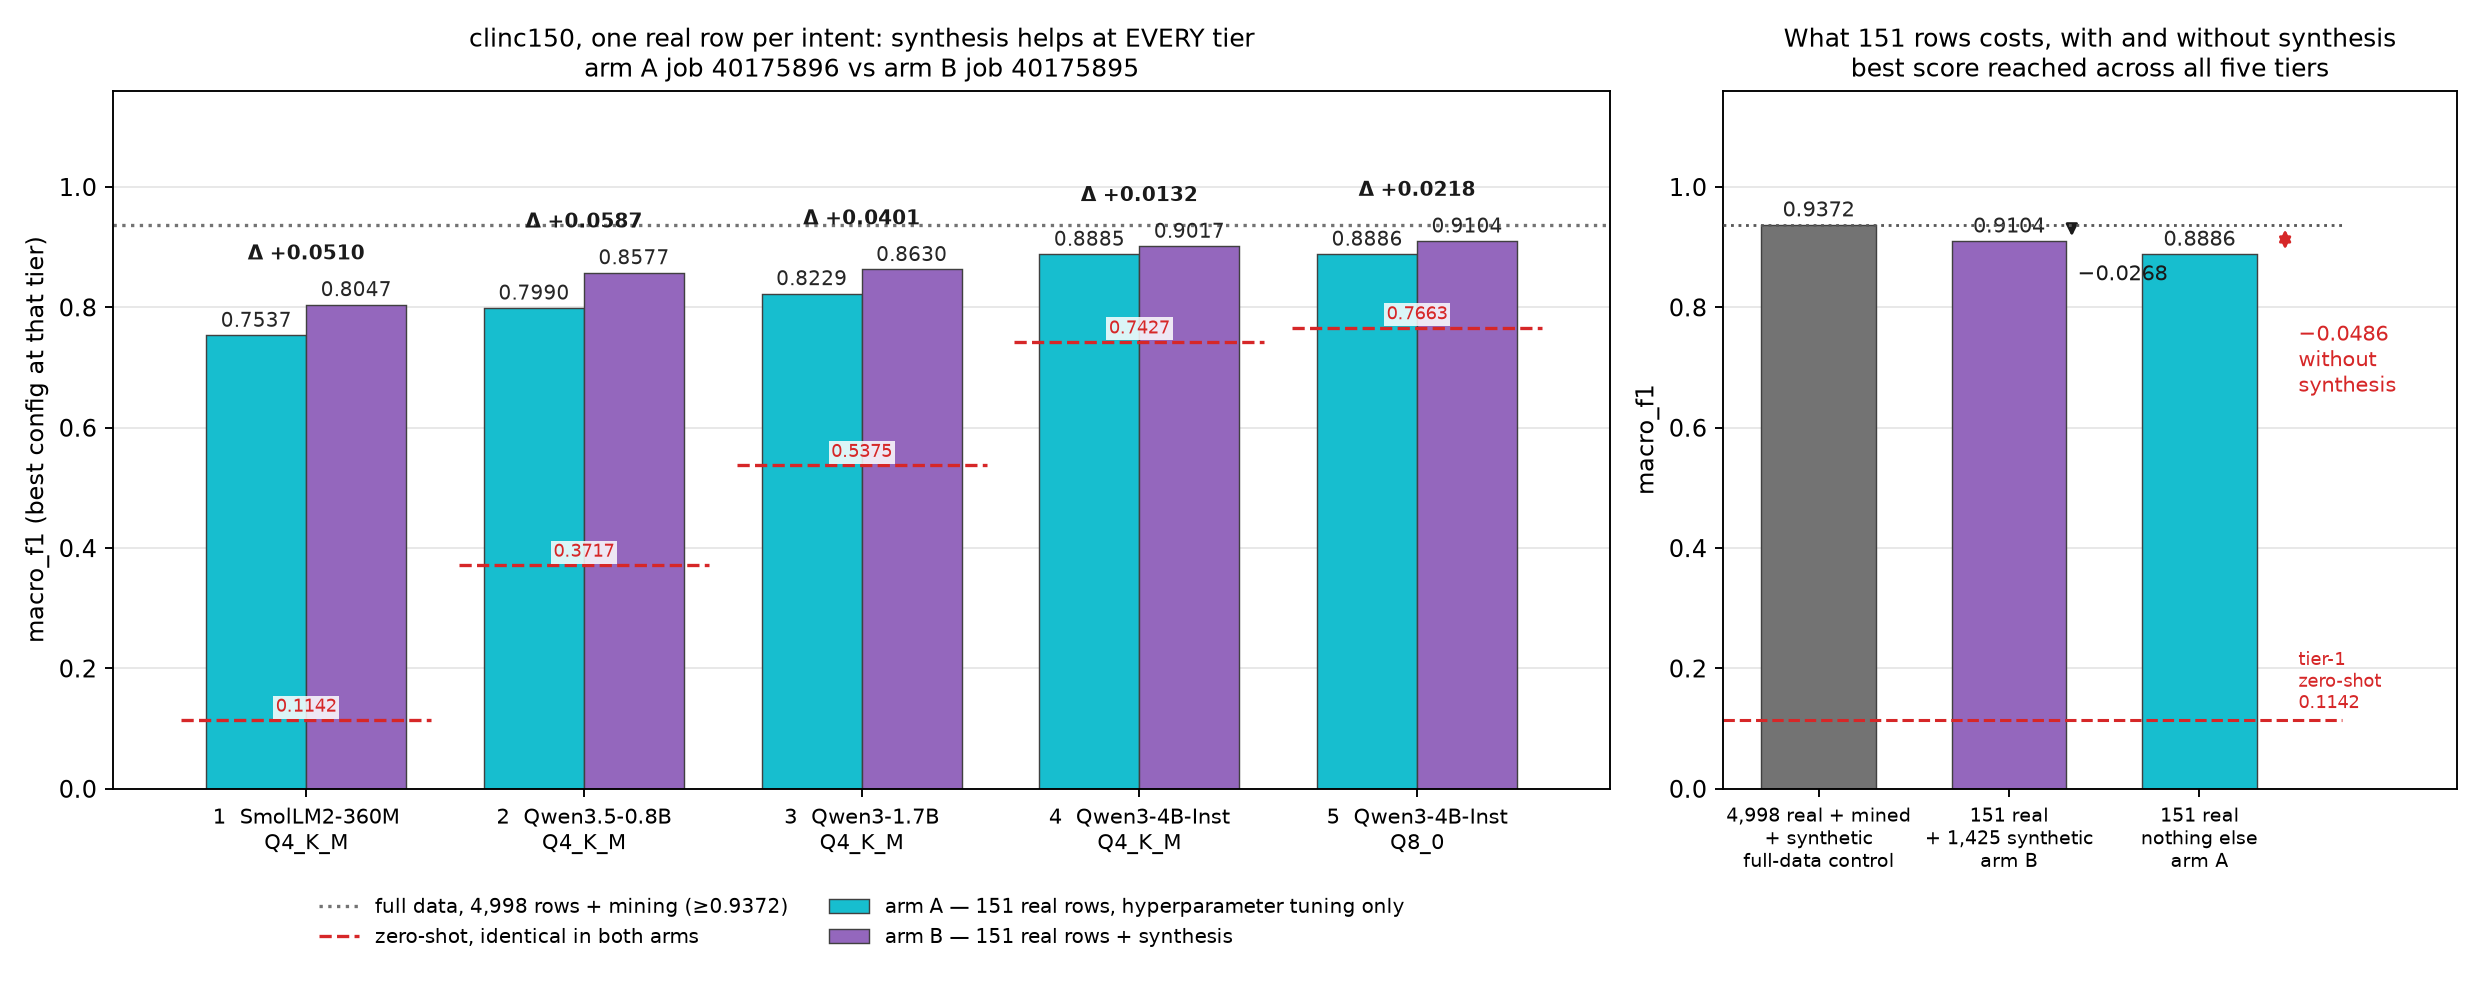
\includegraphics[width=\columnwidth]{figs/clinc150-scarcity-arms.png}
\caption{\tsk{clinc150} scarcity ablation: per-rung bests for both arms against the full-data
control. One real example per intent, 151 classes. \TODO{regenerate at publication DPI;
current figure is a working plot with note-style labelling}}
\label{fig:clinc-scarcity}
\end{figure}

%% The other three existing figures, available in figs/ and not yet placed in the body:
%%   figs/smsspam-scarcity-arms.png     — sms_spam per-rung bests + what synthesis substituted
%%                                        for at 360M (\xref{sec:ablations-scarcity})
%%   figs/synthesis-audit-probes.png    — yield, shadow reject rates, rejection reasons,
%%                                        attempts per kept row (\xref{sec:ablations-synthaudit})
%%   figs/teacher-fewshot-probes.png    — 0-shot vs 5-shot teacher per task
%%                                        (\xref{sec:ablations-fewshot})
%% \TODO{decide which of these three go in the body and which go to an appendix}

\subsection{Does the teacher model change the quality of generated rows?}
\label{sec:ablations-teacher}

Swapping the local 35B teacher for \texttt{deepseek-v4-flash} on \tsk{ner\_bc5cdr}:

\begin{center}
\small
\begin{tabular}{@{}lll@{}}
\toprule
Teacher & \tsk{span\_f1} 5-shot & Format validity \\
\midrule
Qwen3.6-35B-A3B ($\times3$) & 0.3348 / 0.3325 / 0.3299 & \textbf{1.0000} \\
\texttt{deepseek-v4-flash}  & 0.3074                   & \textbf{0.7040} \\
\bottomrule
\end{tabular}
\end{center}

The score gap is small; the format gap is not. Nearly 30\% of the API teacher's NER replies do
not parse as the task's output contract, and an independent measurement on \tsk{xlam\_bfcl}
agrees ($0.679$ arg-match at $0.763$ format validity). On format-bound tasks that is the more
consequential difference.

\textbf{The cause was ours, and we report it as such.} Our synthesis client sent the
thinking-disable flag only on the local path, so the API teacher reasoned on every row: about
7{,}100 output tokens per generated row, \$22.63 of the ablation suite's \$28.84 total and the
whole \$38.05 synthesis bill of the main \tsk{xlam\_bfcl} run (Table~\ref{tab:cost}). Reasoning
text leaking into replies is exactly how a strict output contract fails 30\% of the time. The
judge client had the identical gap while requesting 8 output tokens, so any API-mode run of a
judged task before that fix is suspect. This arm should therefore be read as measuring
\emph{our client}, not the provider, and it needs a re-run before we draw any conclusion about
DeepSeek. We keep it in the paper because the failure mode --- a provider-specific reasoning
flag silently inverting a format-validity result, at 8$\times$ the cost --- is a real hazard
for anyone building this kind of loop. The companion arm that would have measured the
reverse swap --- the local teacher on \tsk{xlam\_bfcl} --- never executed: its job sat
\texttt{PENDING} for roughly 40 hours and was then displaced by a maintenance reservation.

Worth noting separately: the three identical Qwen measurements above span $0.0049$ on the same
model, prompt, and eval set. \emph{The number that gates synthesis and sets the run's goal is
not deterministic.}

\subsection{What do converged tasks reach if not allowed to stop?}
\label{sec:ablations-nostop}

\tsk{clinc150} and \tsk{sms\_spam} were the only suite tasks that ever met their goal --- in 4
and 7 iterations, both at R1 --- so the suite had no measurement of their ceilings. Pinning
the goal at the $0.99$ ceiling makes convergence unreachable and forces the full ladder:

\begin{center}
\small
\begin{tabular}{@{}llll@{}}
\toprule
Task & Original run & No-convergence rerun & Best from \\
\midrule
\tsk{sms\_spam} & 0.9440, 7 it., R1 & \textbf{0.9609}, 85 it., 5 rungs & R3 \\
\tsk{clinc150}  & 0.8952, 4 it., R1 & \textbf{0.9372}, 91 it., 5 rungs & R5 \\
\bottomrule
\end{tabular}
\end{center}

Both are the numbers Table~\ref{tab:main} reports, and both carry caveats we want in the
paper rather than in a footnote. \tsk{sms\_spam}'s peak is at R3 while its \emph{final}
deployed rung scored $0.9490$ --- the ladder overshot its own best, which is a real failure of
the downward probe not being reachable under \texttt{smallest\_first}. And \tsk{clinc150}'s
$0.9372$ is a \emph{lower bound}: that run died at 1d13h on an infrastructure error at R5
iteration 17 with its best set at iteration 16 and still improving. A GGUF conversion exceeded
a flat 600-second ceiling on a merged 4B checkpoint while two other runs were writing
multi-gigabyte checkpoints to the same shared scratch filesystem; the ceiling now scales with
source size and retries once.

\paragraph{Confounds we recommend carrying into any re-run.} Pinning the threshold does not
disable the orchestrator raising it --- one arm pinned to $0.80$ raised itself to $0.85$
anyway, so comparable endpoints need the raise mechanism disabled as well as the threshold
pinned. And stopping at a goal is not the same as reaching a ceiling: three arms stopped the
moment they touched $0.8000$ while the baseline raised its own goal and pushed to $0.8532$,
so comparing endpoints there measures the stretch-goal mechanism and only per-rung numbers are
comparable.

\subsection{Demonstrations, and what the teacher can and cannot do}
\label{sec:ablations-fewshot}

\begin{table}[t]
\centering
\small
\caption{Local teacher, zero- versus five-shot, through each task's own scorer on its frozen
eval set. The empty-output column is the number of rows on which the teacher returned nothing
parseable.}
\label{tab:fewshot}
%% PROVENANCE: 09-16 note Part IV.3, probe jobs on 09-09 and 09-13.
\begin{tabular}{@{}llrrr@{}}
\toprule
Task & Metric & 0-shot & 5-shot & Empty \\
\midrule
\tsk{topv2}          & \tsk{exact\_match}    & 0.0230 & \textbf{0.1290} & 0 / 1000 \\
\tsk{sms\_spam}      & \tsk{minority\_f1}    & 0.8641 & \textbf{0.9213} & 0 / 1000 \\
\tsk{clinc150}       & \tsk{macro\_f1}       & 0.8771 & \textbf{0.9064} & 0 / 1000 \\
\tsk{xlam\_bfcl}     & \tsk{ast\_arg\_match} & 0.8660 & --- & 15 / 1000 \\
\tsk{gec\_bea19}     & \tsk{errant\_f05}     & 0.5014 & --- & 0 / 1000 \\
\tsk{multiconer}     & \tsk{micro\_f1}       & 0.4306 & --- & \textbf{262 / 871} \\
\tsk{goemotions}     & \tsk{ekman\_macro\_f1}& 0.4227 & --- & 21 / 1000 \\
\tsk{dialogsum}      & \tsk{rouge\_l}        & 0.2843 & --- & 0 / 500 \\
\tsk{calendar\_json} & \tsk{ast\_arg\_match} & 0.2037 & --- & \textbf{371 / 535} \\
\tsk{ner\_bc5cdr}    & \tsk{span\_f1}        & 0.1321 & --- & \textbf{600 / 1000} \\
\bottomrule
\end{tabular}
\end{table}

\paragraph{Demonstrations are worth most where the output contract is hardest to guess}
(Table~\ref{tab:fewshot}) ---
\tsk{topv2} $+0.106$ ($5.6\times$), \tsk{sms\_spam} $+0.057$, \tsk{clinc150} $+0.029$ --- in
the same ordering as the empty-output column. The shot ladder on \tsk{topv2} is convex rather
than saturating: $0.0139$ at 0-shot, $0.0203$ at 1, $0.0748$ at 3, $0.1934$ at 5. Nothing
in that curve suggests five is the right number; five is the value the system uses because it
is where we stopped measuring, and we state it that way rather than implying it was tuned.

\paragraph{Three zero-shot cells are depressed for a format reason, not a capability one.}
The teacher returned nothing at all on 600/1000 \tsk{ner\_bc5cdr} rows, 371/535
\tsk{calendar\_json} rows, and 262/871 \tsk{multiconer} rows. The frontier APIs had no such
problem. This is why the fitness gate measures five-shot: a zero-shot number on a
format-bound task mostly reports whether the teacher guessed our contract.

\subsection{Synthesis audit: row quality is a property of the task, not the generator}
\label{sec:ablations-synthaudit}

Ten probe jobs drove the production synthesis path against the local teacher, asking for 60
rows per task and recording yield, programmatic-verifier rejections, and --- in a shadow mode
that keeps every row --- what the teacher-as-verifier \emph{would} have rejected.

\begin{center}
\small
\begin{tabular}{@{}lr@{}}
\toprule
Task & Teacher would reject (\%, range over 9 jobs) \\
\midrule
\tsk{topv2}      & 42.1 -- 66.7 \quad (mean 54) \\
\tsk{multiconer} & 13.6 -- 51.7 \\
\tsk{gec\_bea19} & 0.0 -- 6.7 \\
\tsk{goemotions} & 0.0 \\
\tsk{dialogsum}  & 0.0 \\
\bottomrule
\end{tabular}
\end{center}

On the two structured-parse tasks the teacher would discard between a seventh and two thirds
of what it had just written; \tsk{topv2} never drops below 42\% across nine independent jobs.
On the free-text and label-set tasks it rejects essentially nothing. \emph{Generated-row
quality is a property of the task's output contract, not of the generator.} Every row was
kept anyway, which is what shadow mode means, so \tsk{topv2}'s 824 synthetic rows in
Table~\ref{tab:main}'s run should be read as roughly 450 rows the teacher itself would not
have accepted. Yield ran 32--60 out of 60 requested at $1.2$--$1.6$ generation attempts per
kept row.

The pre-teacher programmatic rejections name specific, actionable defects: on \tsk{topv2},
59 rows whose parse leaves do not reproduce the command word-for-word
(``remind me to milk'' for ``remind me to buy milk''), 49 intents labelled with no spans at
all, 33 labels outside the closed vocabulary, 20 malformed trees; on \tsk{multiconer}, 24
plausible synonyms for real classes (\texttt{OtherORG}, \texttt{Location}, \texttt{Loc})
against a scorer that compares labels exactly; on \tsk{dialogsum}, 107 rows carrying two or
three references when a generated row has one author, which is a schema mismatch rather than
a quality problem.

\paragraph{The teacher is a bad student and a decent generator, on different tasks.}
It scores $0.023$ on \tsk{topv2} zero-shot and $0.129$ with five demonstrations, yet writes
\tsk{topv2} rows its own programmatic verifier accepts 90\% of the time. Generating a labelled
example and answering a held-out one are not the same capability --- and our fitness gate
measures only the second. We consider this the clearest known design flaw in the gate.

\subsection{Mining: no task ever gained a row from a new external source}

Across the suite, zero tasks acquired a row from web discovery --- and not for lack of
candidates. On \tsk{ner\_bc5cdr} the search found eight BC5CDR datasets and six were rejected
by a comparison that cannot succeed: a discovery registry recorded BC5CDR's task as
\texttt{"NER"} while the task registry name is \tsk{ner\_bc5cdr}, and the gate rejects on
inequality. One more was skipped because the hub dropped loading-script support and one failed
for a real schema reason. Two such rounds retire mining permanently. Fixing it would mostly
buy duplicates of the same corpus; the tasks that would benefit from a genuinely different
source are the thin ones. We report it because a null result produced by a string comparison
is not a null result about mining.

\subsection{Controls that exist but have no comparable endpoint}

Three of the system's ablation controls are implemented and, in one case, observed firing
correctly, but none has produced a paired measurement. We list them so that the scope of the
evidence above is unambiguous.

\squishlist
\item \textbf{The ladder itself.} \texttt{single\_model} is implemented as the control that
isolates what escalation buys, and is enforced at all three ladder gates, but no paired
\texttt{single\_model} versus \texttt{smallest\_first} run exists. The claim in
\xref{sec:results} that the ladder accounts for more of the improvement than the search does
therefore rests on the \emph{decomposition} of the observed runs --- per-rung search gains in
Table~\ref{tab:main} against between-rung differences in Table~\ref{tab:scarcity} --- and not
on a controlled comparison.
\item \textbf{Curriculum reset on escalation.} The mechanism fires correctly at a rung
promotion (observed: ``Dataset RESET to seed: v2 $\to$ v3, 2621 $\to$ 2603 rows''), but the
arm carrying it converged at R2 and stopped, so no effect on final score can be read off it.
\item \textbf{Rollback on and off.} No such pair exists. The role we ascribe to rollback in
\xref{sec:results} --- converting a 19\% intervention hit rate into monotone progress --- is
an argument from the mechanism and from the per-iteration tables, not a measured contrast.
\squishend

%% ====================================================================
\section{How Reliably Can Any of This Be Measured?}
\label{sec:reliability}

\subsection{Training is not bit-reproducible}

The \tsk{clinc150} scarcity arms' first fine-tunes ran on the same MD5-identical 151-row file,
the same configuration, batch and learning-rate schedule, a seeded LoRA initialization, a
seeded shuffle, identical peak memory (2{,}592\,MiB), and greedy decoding --- and finished at
training loss $1.096$ against $1.093$, scoring $0.2781$ against $0.2934$. Their recorded
effective configurations differ in exactly two keys: the ablation switch and a log path.

A dedicated probe established the cause: training the same file twice with identical arguments
produced two different adapters (SHA-256 \texttt{933f037f\dots} against
\texttt{f6c9ba31\dots}). Nothing in the harness had asked for determinism, so \texttt{bf16}
reduction order followed runtime scheduling. We fixed what can be fixed --- seeds,
\texttt{CUBLAS\_WORKSPACE\_CONFIG}, cuDNN flags, and
\texttt{use\_deterministic\_algorithms}, all applied centrally and logged by every run --- and
it does \emph{not} make training bit-exact: four further probes still produced differing
adapters, including across separate processes and with \texttt{torch.compile} disabled.
PyTorch emits no nondeterminism warnings, so the residue is in the fused kernels of our
training library, which that flag does not reach.

\subsection{Quantization amplifies it}

\begin{table}[t]
\centering
\small
\caption{The same two independently-trained adapters, scored three ways on identical rows.
Training nondeterminism is worth about $0.001$; 4-bit quantization multiplies it roughly
fivefold; a small selection eval multiplies it again.}
\label{tab:determinism}
%% PROVENANCE: 09-16 note Part III.3; probes 40254317, 40254741, 40253558/685/741/871.
\begin{tabular}{@{}lrrr@{}}
\toprule
Scoring configuration & Arm 1 & Arm 2 & Gap \\
\midrule
\texttt{bf16}, 5{,}500-row report split      & 0.3403 & 0.3390 & \textbf{0.0013} \\
\texttt{Q4\_K\_M}, 5{,}500-row report split  & 0.2798 & 0.2859 & \textbf{0.0061} \\
\texttt{Q4\_K\_M}, 1{,}000-row in-loop eval  & 0.2781 & 0.2934 & \textbf{0.0153} \\
\bottomrule
\end{tabular}
\end{table}

Table~\ref{tab:determinism} scores the same two independently-trained adapters three ways.
Rounding to 4 bits is a threshold operation, so weights differing in their last bits land in
different buckets: format validity moved $0.755$ against $0.740$ under \texttt{Q4\_K\_M} where
in \texttt{bf16} it moved $0.657$ against $0.655$. The 1{,}000-row in-loop eval multiplies it
again, because macro-F1 over 151 classes has roughly 6.6 eval rows per class there against 36
on the report split.

Two consequences, both of which we apply throughout the paper. A per-rung margin near
$\pm0.015$ is not attributable to an experimental arm, so the \tsk{clinc150} scarcity claim
rests on the sign being the same at all five rungs and four of them clearing that band. And
\emph{paper numbers come from the standalone report script, not from the in-loop figure}: the
same nondeterminism costs $0.0013$ there against $0.0153$ in the loop.

\subsection{The noise floor}

The $\pm0.015$ floor quoted throughout is measured, not assumed. Three probe jobs ran the same
two tasks three times with nothing varied: \tsk{sms\_spam} zero-shot moved
$0.8552 / 0.8641 / 0.8834$, a $0.0282$ spread with no demonstrations to vary. Independently,
the teacher fitness measurement jitters $0.0049$ across three identical runs. We treat any
single-run difference below that band as unmeasured, and we recommend that any system
reporting agentic fine-tuning deltas publish an equivalent triplicate.

%% ====================================================================
\section{Discussion}
\label{sec:discussion}

\paragraph{The ladder does more than the search, and that reframes what the agent is for.}
Table~\ref{tab:main} shows the post-first-fine-tune search gain is a median $+0.033$ while the
between-rung differences in Table~\ref{tab:scarcity} run to $0.3$ and more. If the goal were
accuracy alone, the honest summary would be ``pick a bigger model.'' It is the
footprint constraint that makes the search valuable: at a fixed rung --- which is what a phone
imposes --- the search is the only lever, and the scarcity ablation shows it is worth
$+0.298$ at the rung that a small device forces you onto.

\paragraph{The system's most useful outputs are sometimes negative.} \tsk{dialogsum} produced
$+0.0000$ over 15 iterations at its best rung, and the correct output of the loop is ``ship the
base model.'' \tsk{clinc150} behaves as an in-distribution control where the loop adds little.
\tsk{xlam\_bfcl} is a loss against both frontier APIs. We report these as results because a
closed-loop system that cannot say ``nothing to do here'' will always find something to do,
and the zero-shot-competes-as-a-candidate rule is the mechanism that lets it say so.

\paragraph{Honesty mechanisms paid for themselves in bugs caught.} Separating content from
format score revealed a checkpoint emitting stray reasoning tags that had corrupted two runs.
Recording failed measurements as \texttt{n/a} rather than $0.0$ retracted a fabricated
$+0.85$ improvement. Keying the GGUF cache on quantization method as well as weights caught
two rungs silently scoring the same file. Deriving failure categories from the scorer stopped
the orchestrator reasoning about a constant. None of these were found by tests; all were found
by making the report state what was actually measured.

\paragraph{What we would tell someone building this.} Make the deployment artifact the thing
you score. Make every threshold require a repeat or a magnitude that variance cannot explain.
Never let an estimated quantity enter a gate in the same shape as a measurement. And measure
your own noise floor before you believe any delta, including your own.

%% ====================================================================
\section{Limitations}
\label{sec:limitations}

\paragraph{No on-phone runtime measurement.} This is the most important limitation.
The hardware constraint model gates on measured on-disk weight bytes against usable RAM and
storage, which is a necessary but not sufficient condition for running on a device. We have
not measured tokens per second, time to first token, peak resident set, or power on any
physical phone: the runtime measurement table in our repository is empty, and the measurement
harness exists but has not been run against target hardware. Accordingly we make no
throughput, latency, or battery claim anywhere in this paper, and the ``deployable'' claim
should be read as ``the weights fit, and the quantized artifact was scored in the numerical
format it would be served in.'' Everything in this paper is therefore a statement about
deployability under a memory budget, not about on-device latency or energy.

\paragraph{Quantized evaluation runs on server hardware.} GGUF scoring uses
\texttt{llama.cpp} with a CUDA build on an L40S, not an Arm SoC. The numerical result of a
\texttt{Q4\_K\_M} forward pass should be near-identical, but we have not verified that the
same artifact scores the same on-device.

\paragraph{Production mode is absent.} The prior system we build on
contributes a production mode driven by judged inference failures. We architected the
corresponding entry chain, never wired it into the graph topology, and removed it. Every
result here is cold-start. A continual-improvement claim would need the flywheel, a regression
gate, and a replay buffer that we designed but did not ship.

\paragraph{One seed per arm.} Given \xref{sec:reliability}, single-seed arms are a real
weakness. The scarcity claims rest on the sign of the effect being consistent across all five
rungs, and on four of five clearing the measured noise band, rather than on any single margin.
No arm in this paper is replicated.

\paragraph{Five of ten suite runs bypassed the teacher fitness gate.} Stated in
\xref{sec:suite}. Those runs are not clean in the gate's own terms.

\paragraph{One of ten suite runs used a different teacher.} \tsk{xlam\_bfcl} ran with
\texttt{deepseek-v4-flash} rather than the local Qwen3.6 endpoint, so its synthetic rows were
produced under a different generator --- and, because of the reasoning-flag bug in
\xref{sec:ablations-teacher}, a badly behaved one. That run's synthesis is not comparable to
the other nine, and it is also the suite's only loss against the frontier APIs. We do not
claim those two facts are linked, but nothing in our data rules the link out.

\paragraph{The fitness gate measures the wrong capability.} It scores the teacher as a
\emph{student} on the task, but uses the teacher as a \emph{generator}.
\xref{sec:ablations-synthaudit} shows those diverge sharply: the teacher scores $0.023$ on
\tsk{topv2} and writes rows its own verifier accepts 90\% of the time. A generation-side gate
is the obvious fix and is not implemented.

\paragraph{Synthesis has never run at scale in a fully clean completed run.} Endpoint
availability and, in one case, a dispatch bug that silently produced zero rows mean that
several of our synthesis-quality claims rest on probes rather than on production runs.

\paragraph{Mining never contributed an external row}, for the string-comparison reason in
\xref{sec:ablations}. The mining ladder is therefore effectively a re-read of known corpora in
every result here.

\paragraph{The downward probe is unreachable under the default strategy.} It is reachable only
from \texttt{interpolation} and \texttt{orchestrator\_choice}, and every suite run used
\texttt{smallest\_first}. This is why \tsk{sms\_spam} deployed at R5 ($0.9490$) when its best
was at R3 ($0.9609$) --- the second half of Equation~\ref{eq:objective} did not run. The
footprint-minimizing half of our objective is therefore stated but not exercised in any
result reported here, and the ladder's terminal rung should be read as ``where the run
stopped'' rather than as ``the smallest variant that clears $\theta$.''

\paragraph{Contamination is bounded structurally, not measured.} Our tasks are public
benchmarks and our frontier baselines may have seen them. We enforce train/eval separation
rigorously within a run; we make no claim about pretraining exposure.

%% ====================================================================
\section{Conclusion}

Making a language model useful on a specific phone for a specific job is a constrained search
problem, and the constraint is the interesting part. SLM Factory treats the deployment
artifact's measured footprint as the objective and a teacher-calibrated accuracy target as the
constraint, searches jointly over training pipelines and quantized deployment variants, and
scores every candidate as it would actually be served. On a ten-task suite the resulting
on-device students beat two frontier APIs zero-shot on nine tasks, with the decisive wins on
format-bound tasks where the base model scores near zero and where two of the three winning
artifacts ship under 1.3\,GB. Equally, the loop's iterative search contributes a median of
$+0.033$ after the first fine-tune, 81\% of its interventions are rolled back, and synthetic data is
worth $+0.05$ per rung under scarcity and nothing at all when real data is plentiful. We
report both halves, along with the measurement work showing that fine-tuning under our stack
is not bit-reproducible and that 4-bit quantization amplifies that nondeterminism fivefold,
because a system that only reports its wins cannot be used to decide anything.

%% ====================================================================
%% \TODO{Appendices to write:
%%   A. Full per-iteration tables for all ten suite runs (curriculum growth, QC removals,
%%      verification keep rate, score, delta, kept/rolled-back).
%%   B. The five tunable hyperparameters and the fixed training choices, with the reasoning
%%      for each retirement (batch shape trainer-derived, dropout pinned at 0).
%%   C. Prompt appendix: task brief authoring, intervention decision, model selection,
%%      threshold raise, synthesis, verification. All six are in docs/PROMPTS.md.
%%   D. The run-health watchdog thresholds and the incident behind each.
%%   E. Reproduction: the two determinism probe scripts.
%% }

\begin{thebibliography}{99}
\small

%% \TODO{This is a hand-rolled bibliography so the draft compiles standalone. Convert to
%% refs.bib + ACM-Reference-Format before submission. Several entries are placeholders with
%% plausible-but-unverified venue/year fields and are marked CHECK.}

\bibitem{atreja2026pioneer}
D. Atreja, J. White, N. Nayak, K. Zhang, H. Princis, G. Hurn-Maloney, A. Lewis, and
U. Zaratiana. Pioneer Agent: Continual improvement of small language models in production.
\emph{arXiv:2604.09791}, 2026.

\bibitem{hu2021lora}
E. J. Hu, Y. Shen, P. Wallis, Z. Allen-Zhu, Y. Li, S. Wang, L. Wang, and W. Chen.
LoRA: Low-rank adaptation of large language models. \emph{ICLR}, 2022.

\bibitem{dettmers2023qlora}
T. Dettmers, A. Pagnoni, A. Holtzman, and L. Zettlemoyer. QLoRA: Efficient finetuning of
quantized LLMs. \emph{NeurIPS}, 2023.

\bibitem{dettmers2022llmint8}
T. Dettmers, M. Lewis, Y. Belkada, and L. Zettlemoyer. LLM.int8(): 8-bit matrix
multiplication for transformers at scale. \emph{NeurIPS}, 2022.

\bibitem{frantar2022gptq}
E. Frantar, S. Ashkboos, T. Hoefler, and D. Alistarh. GPTQ: Accurate post-training
quantization for generative pre-trained transformers. \emph{ICLR}, 2023.

\bibitem{lin2024awq}
J. Lin, J. Tang, H. Tang, S. Yang, X. Dang, and S. Han. AWQ: Activation-aware weight
quantization for LLM compression and acceleration. \emph{MLSys}, 2024.

\bibitem{feurer2015autosklearn}
M. Feurer, A. Klein, K. Eggensperger, J. Springenberg, M. Blum, and F. Hutter. Efficient and
robust automated machine learning. \emph{NeurIPS}, 2015.

\bibitem{thornton2013autoweka}
C. Thornton, F. Hutter, H. H. Hoos, and K. Leyton-Brown. Auto-WEKA: Combined selection and
hyperparameter optimization of classification algorithms. \emph{KDD}, 2013.

\bibitem{feurer2019automl}
M. Feurer and F. Hutter. Hyperparameter optimization. In \emph{Automated Machine Learning},
Springer, 2019.

\bibitem{bergstra2012random}
J. Bergstra and Y. Bengio. Random search for hyper-parameter optimization. \emph{JMLR},
13:281--305, 2012.

\bibitem{elsken2019nas}
T. Elsken, J. H. Metzen, and F. Hutter. Neural architecture search: A survey. \emph{JMLR},
20(55):1--21, 2019.

\bibitem{cai2019proxylessnas}
H. Cai, L. Zhu, and S. Han. ProxylessNAS: Direct neural architecture search on target task
and hardware. \emph{ICLR}, 2019.

\bibitem{wu2019fbnet}
B. Wu, X. Dai, P. Zhang, Y. Wang, F. Sun, Y. Wu, Y. Tian, P. Vajda, Y. Jia, and K. Keutzer.
FBNet: Hardware-aware efficient ConvNet design via differentiable neural architecture search.
\emph{CVPR}, 2019.

\bibitem{tan2019mnasnet}
M. Tan, B. Chen, R. Pang, V. Vasudevan, M. Sandler, A. Howard, and Q. V. Le. MnasNet:
Platform-aware neural architecture search for mobile. \emph{CVPR}, 2019.

\bibitem{chan2024mlebench}
J. S. Chan et al. MLE-bench: Evaluating machine learning agents on machine learning
engineering. \emph{arXiv:2410.07095}, 2024.

\bibitem{nam2025mlgym}
D. Nam et al. MLGym: A new framework and benchmark for advancing AI research agents.
\emph{arXiv}, 2025. %% CHECK
%% \TODO{verify this citation; I have it second-hand from the Pioneer Agent related-work section}

\bibitem{chen2026kernelagent}
Chen et al. Agentic search for GPU kernel optimization. 2026. %% CHECK — placeholder
%% \TODO{find the real citation or drop}

\bibitem{yamada2025aiscientist}
Y. Yamada et al. The AI Scientist-v2: Workshop-level automated scientific discovery.
\emph{arXiv}, 2025. %% CHECK

\bibitem{gottweis2025coscientist}
J. Gottweis et al. Towards an AI co-scientist. \emph{arXiv:2502.18864}, 2025.

\bibitem{northcutt2021confident}
C. G. Northcutt, L. Jiang, and I. L. Chuang. Confident learning: Estimating uncertainty in
dataset labels. \emph{JAIR}, 70:1373--1411, 2021.

\bibitem{mazumder2023dataperf}
M. Mazumder et al. DataPerf: Benchmarks for data-centric AI development. \emph{NeurIPS
Datasets and Benchmarks}, 2023.

\bibitem{zhou2023lima}
C. Zhou et al. LIMA: Less is more for alignment. \emph{NeurIPS}, 2023.

\bibitem{wang2023selfinstruct}
Y. Wang, Y. Kordi, S. Mishra, A. Liu, N. A. Smith, D. Khashabi, and H. Hajishirzi.
Self-Instruct: Aligning language models with self-generated instructions. \emph{ACL}, 2023.

\bibitem{hinton2015distilling}
G. Hinton, O. Vinyals, and J. Dean. Distilling the knowledge in a neural network.
\emph{arXiv:1503.02531}, 2015.

\bibitem{bansal2025smallerweaker}
H. Bansal et al. Smaller, weaker, yet better: Training LLM reasoners via compute-optimal
sampling. \emph{ICLR}, 2025.

\bibitem{sainz2023nlpcontamination}
O. Sainz, J. A. Campos, I. García-Ferrero, J. Etxaniz, O. L. de Lacalle, and E. Agirre.
NLP evaluation in trouble: On the need to measure LLM data contamination for each benchmark.
\emph{EMNLP Findings}, 2023.

\bibitem{golchin2024timetravel}
S. Golchin and M. Surdeanu. Time travel in LLMs: Tracing data contamination in large language
models. \emph{ICLR}, 2024.

%% \TODO{Still need citations for, at minimum:
%%   - each of the ten benchmarks (CLINC150, SMS Spam, xLAM/BFCL, BC5CDR, GoEmotions,
%%     BEA-2019/ERRANT, MultiCoNER, DialogSum, TOPv2, GSM8K)
%%   - Qwen3 / Qwen3.5 technical reports, SmolLM2, Gemma 3
%%   - Unsloth, PEFT, Transformers, llama.cpp, LangGraph, vLLM
%%   - ROUGE, ERRANT, macro-F1 / minority-F1 conventions
%%   - catastrophic forgetting (Kirkpatrick et al.) if we keep the replay discussion
%%   - calibration (Guo et al.) if we keep the confidence discussion }

\end{thebibliography}

\end{document}

%% ====================================================================
%% OPEN QUESTIONS FOR THE AUTHORS — everything I could not resolve from the repo.
%% Collected here so they are in one place; each also appears inline as a \TODO.
%%
%% IDENTITY
%%  1. Author list, order, affiliations, corresponding email.
%%  2. Target venue and deadline. The style here is ACM sigconf per draft.tex, but the
%%     structure (long methods section, heavy negative-results reporting) reads more like
%%     an arXiv tech report. These want different papers.
%%  3. Project/system name: "SLM Factory" throughout. Keep?
%%  4. Code/artifact release: repo URL, license, whether logs and eval sets ship.
%%
%% FIGURES I NEED
%%  5. Figure 1: system architecture. Needs drawing (tikz or external).
%%  6. Figure 2: score vs measured footprint per rung, all ten tasks. Data exists in the
%%     run logs' per-tier reports; the plot does not.
%%  7. Existing figures to regenerate at publication quality:
%%     docs/Evan's Notes/img/09-16-clinc150-scarcity-arms.png
%%     docs/Evan's Notes/img/09-14-scarcity-ablation-arms.png
%%     docs/Evan's Notes/img/09-16-synthesis-audit-probes.png
%%     docs/Evan's Notes/img/09-16-teacher-fewshot-probes.png
%%  8. Per-run accuracy-vs-iteration panels exist under logs/graphics/<run>/summary.png —
%%     do you want one of these in the body as a trajectory example, or in an appendix?
%%
%% NUMBERS I COULD NOT FIND
%%  9. Wall clock per suite run. I have costs and iteration counts from the logs but not
%%     durations; SLURM accounting has them.
%% 10. The device string / RAM+storage budget used for the suite runs. The ladder's top
%%     rung is 4,082 MB of weights, which implies a generous budget, and the paper should
%%     state what device was claimed.
%% 11. gsm8k and routerbench / proactive_listening / toolbench are in the repo with results
%%     but are not in the "main 10" table. Do they go in an appendix table, or stay out?
%%
%% SCOPE DECISIONS (no new experiments assumed — the paper is written against what is
%% already measured, and every gap is stated as a limitation rather than as future work)
%% 12. Sec. 10 (Limitations) now states each unexercised control as plain scope:
%%       - no on-phone runtime measurement (measurements dict is empty)
%%       - GGUF scoring on server hardware, not an Arm SoC
%%       - no production mode
%%       - one seed per arm, no replication
%%       - five of ten runs bypassed the teacher fitness gate
%%       - xlam_bfcl used a different teacher from the other nine
%%       - the downward probe never executed, so Eq. 2's minimizing half is stated not shown
%%       - mining never contributed an external row
%%     Sec. 7.8 lists the three ablation controls that exist without a paired endpoint.
%%     If you would rather these be cut entirely rather than stated, say so and I will
%%     remove them — but note that several of the paper's claims are scoped by them.
%% 13. Negative results currently occupy roughly a third of the page budget (Sec. 7
%%     ablations, Sec. 8 reliability, and the honest readings under each results table).
%%     That is deliberate and it is what differentiates this from the Pioneer Agent paper.
%% 14. Confirm whether the honesty-mechanisms subsection in Sec. 9 stays in the body.
%% ====================================================================
